\begin{frame}
\frametitle{Interprète}
L'interprète est constitué de 3 analyseurs
\begin{itemize}
\item un analyseur lexical (Flex)
\item un analyseur syntaxique (Bison)
\item un analyseur sémantique (C++)
\end{itemize}
\end{frame}

\subsection{Analyse lexicale}
\begin{frame}
	\frametitle{Analyseur lexical}
	\begin{description}
		\item [Objectif] Génération de jetons
		\item [Méthode] Détection de lexèmes par des expressions régulières
		\item [Outil] GNU Flex (Lex)
	\end{description}
\end{frame}

\begin{frame}[fragile]
	\begin{rail}
		NUMBER : (('0-9' + ) \\ ( (dot ( '0-9' * ) ) ?))
		| dot ( '0-9' + ) ;
	\end{rail}
\end{frame}

\begin{frame}[fragile]
	Code~:
	\begin{lstlisting}[language=Stibbons]
new agent {
  a = 10
  fd a + 2
}
	\end{lstlisting}
	Jetons~:
	\begin{lstlisting}[breaklines]
<NEW> <AGT> <{> <\n> 
<ID,"a"> <=> <NUMBER,10> <\n>
<FD> <ID,"a"> <+> <NUMBER,2> <\n>
<}>
	\end{lstlisting}
\end{frame}


\subsection{Analyse syntaxique}
\begin{frame}
	\begin{itemize}
	\item Objectif double~: 
		\begin{itemize}
		\item Vérifier la validité du programme écrit~;
		\item Générer un arbre abstrait analysable par l'analyseur sémantique.
		\end{itemize}
	\item Langage utilisé~: GNU Bison.
	\end{itemize}
\end{frame}

\begin{frame}
L'exemple précédent génère l'abre abstrait suivant~:
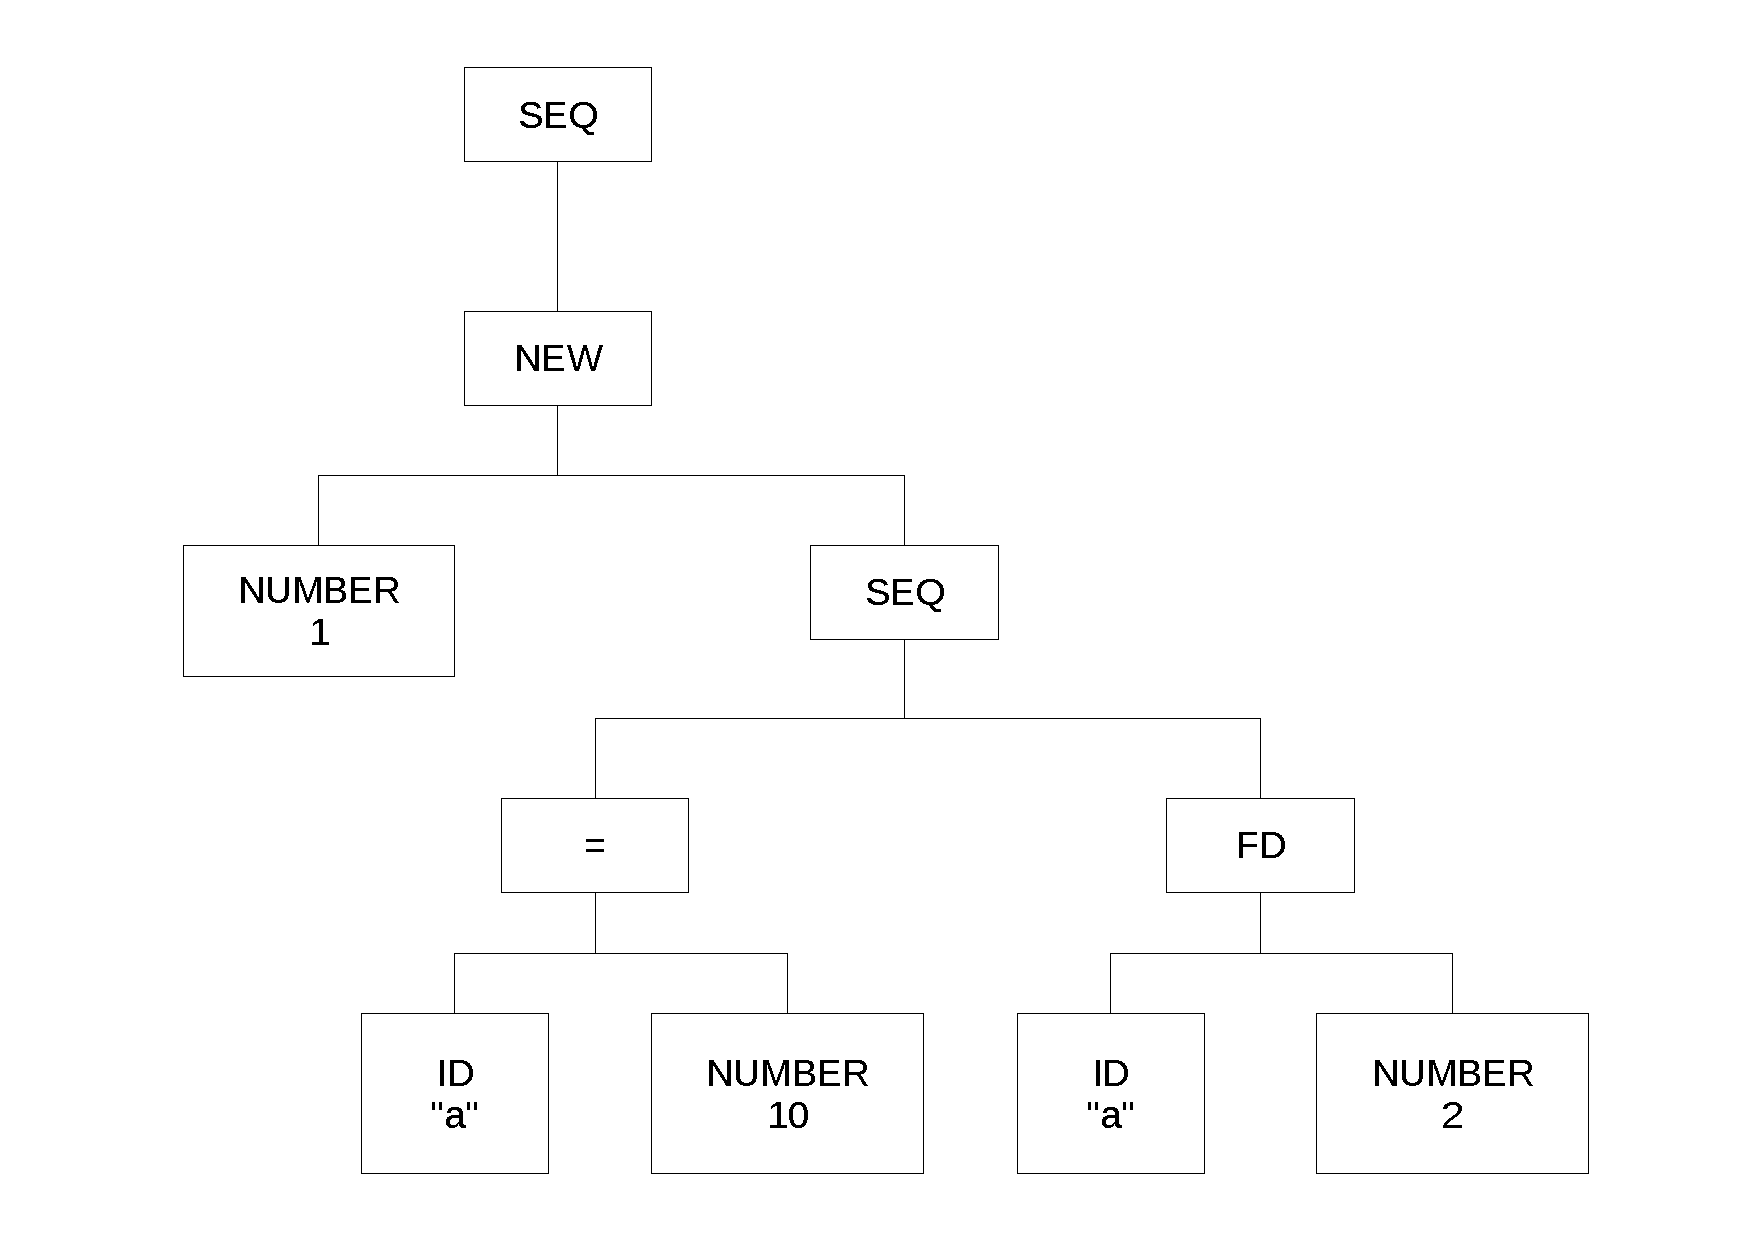
\includegraphics[scale=0.3]{doc/Presentation/img/arbre.pdf}
\end{frame}



\subsection{Analyse sémantique}

\begin{frame}
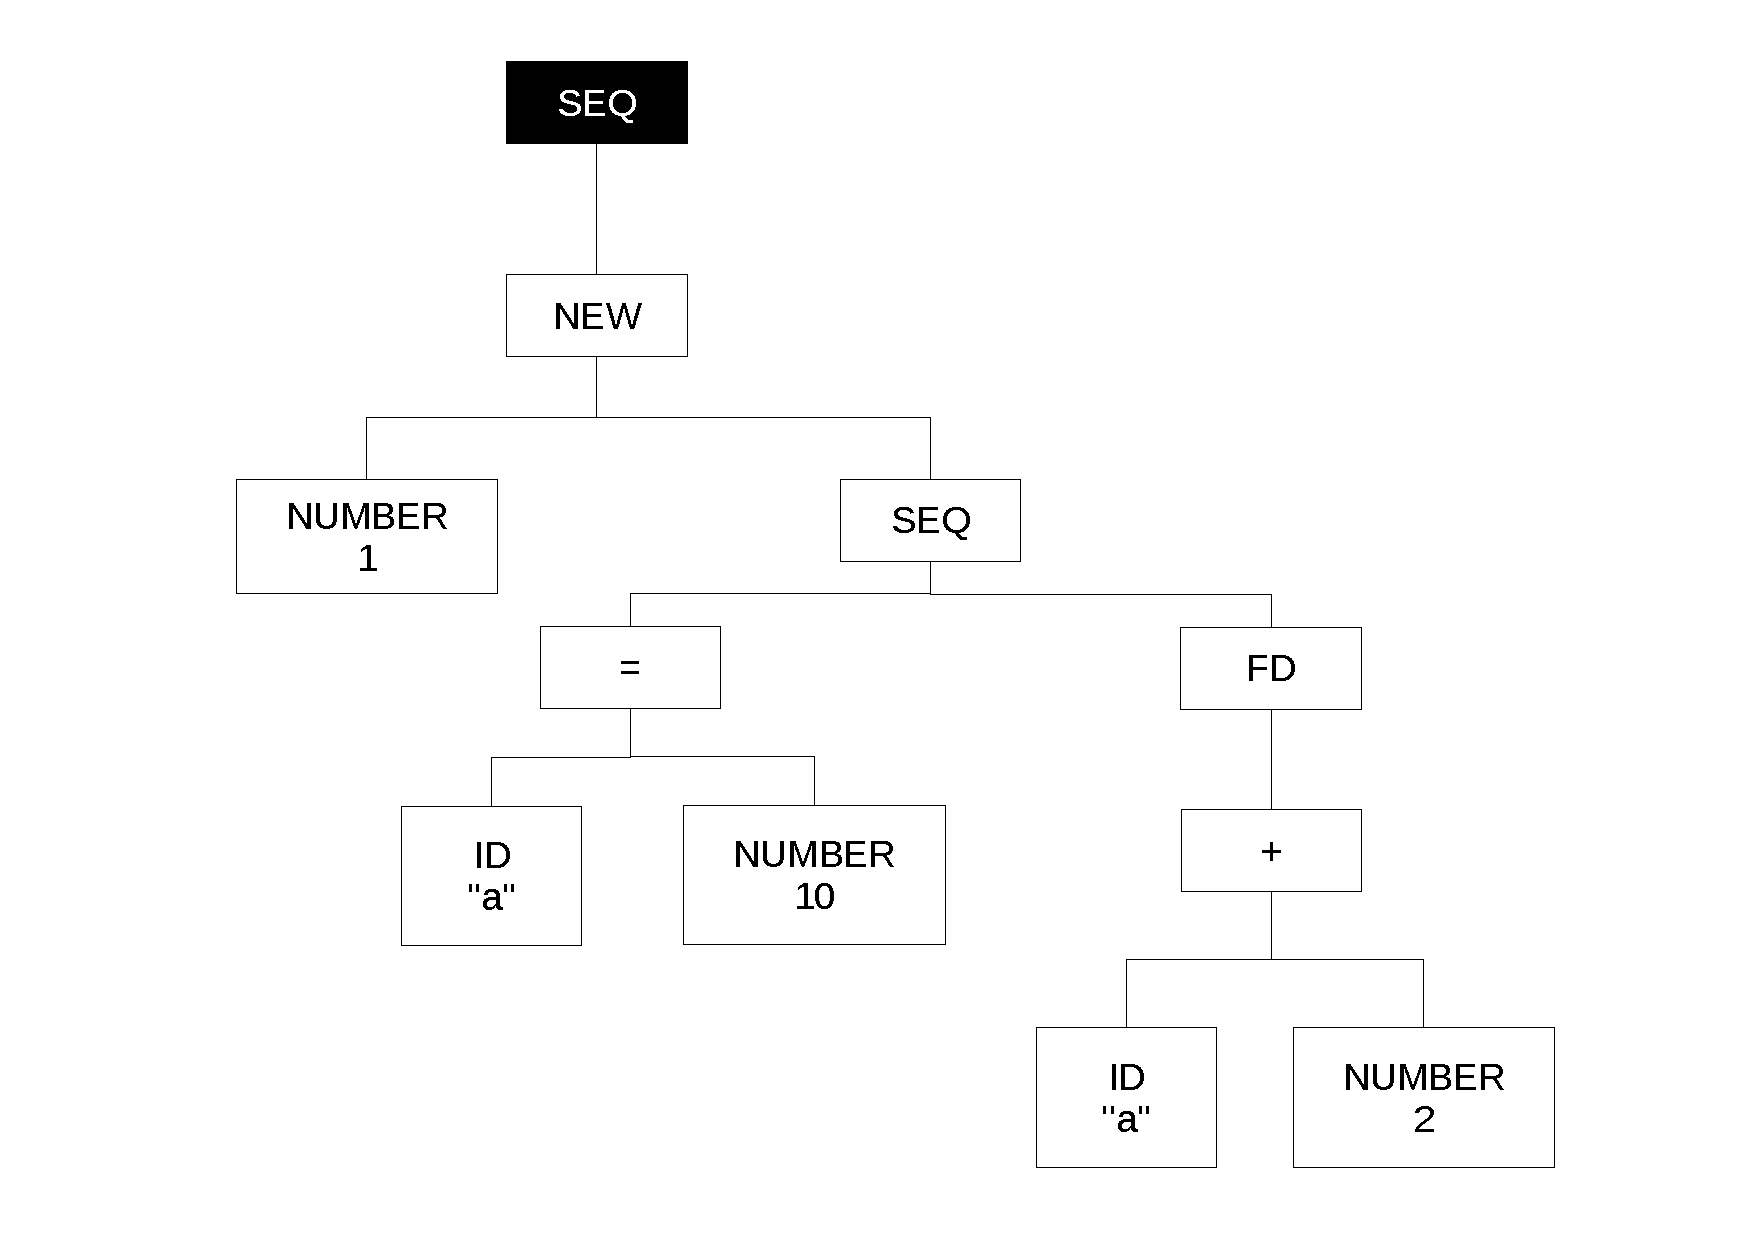
\includegraphics[scale=0.3]{doc/Presentation/img/arbre1.pdf}
\end{frame}

\begin{frame}
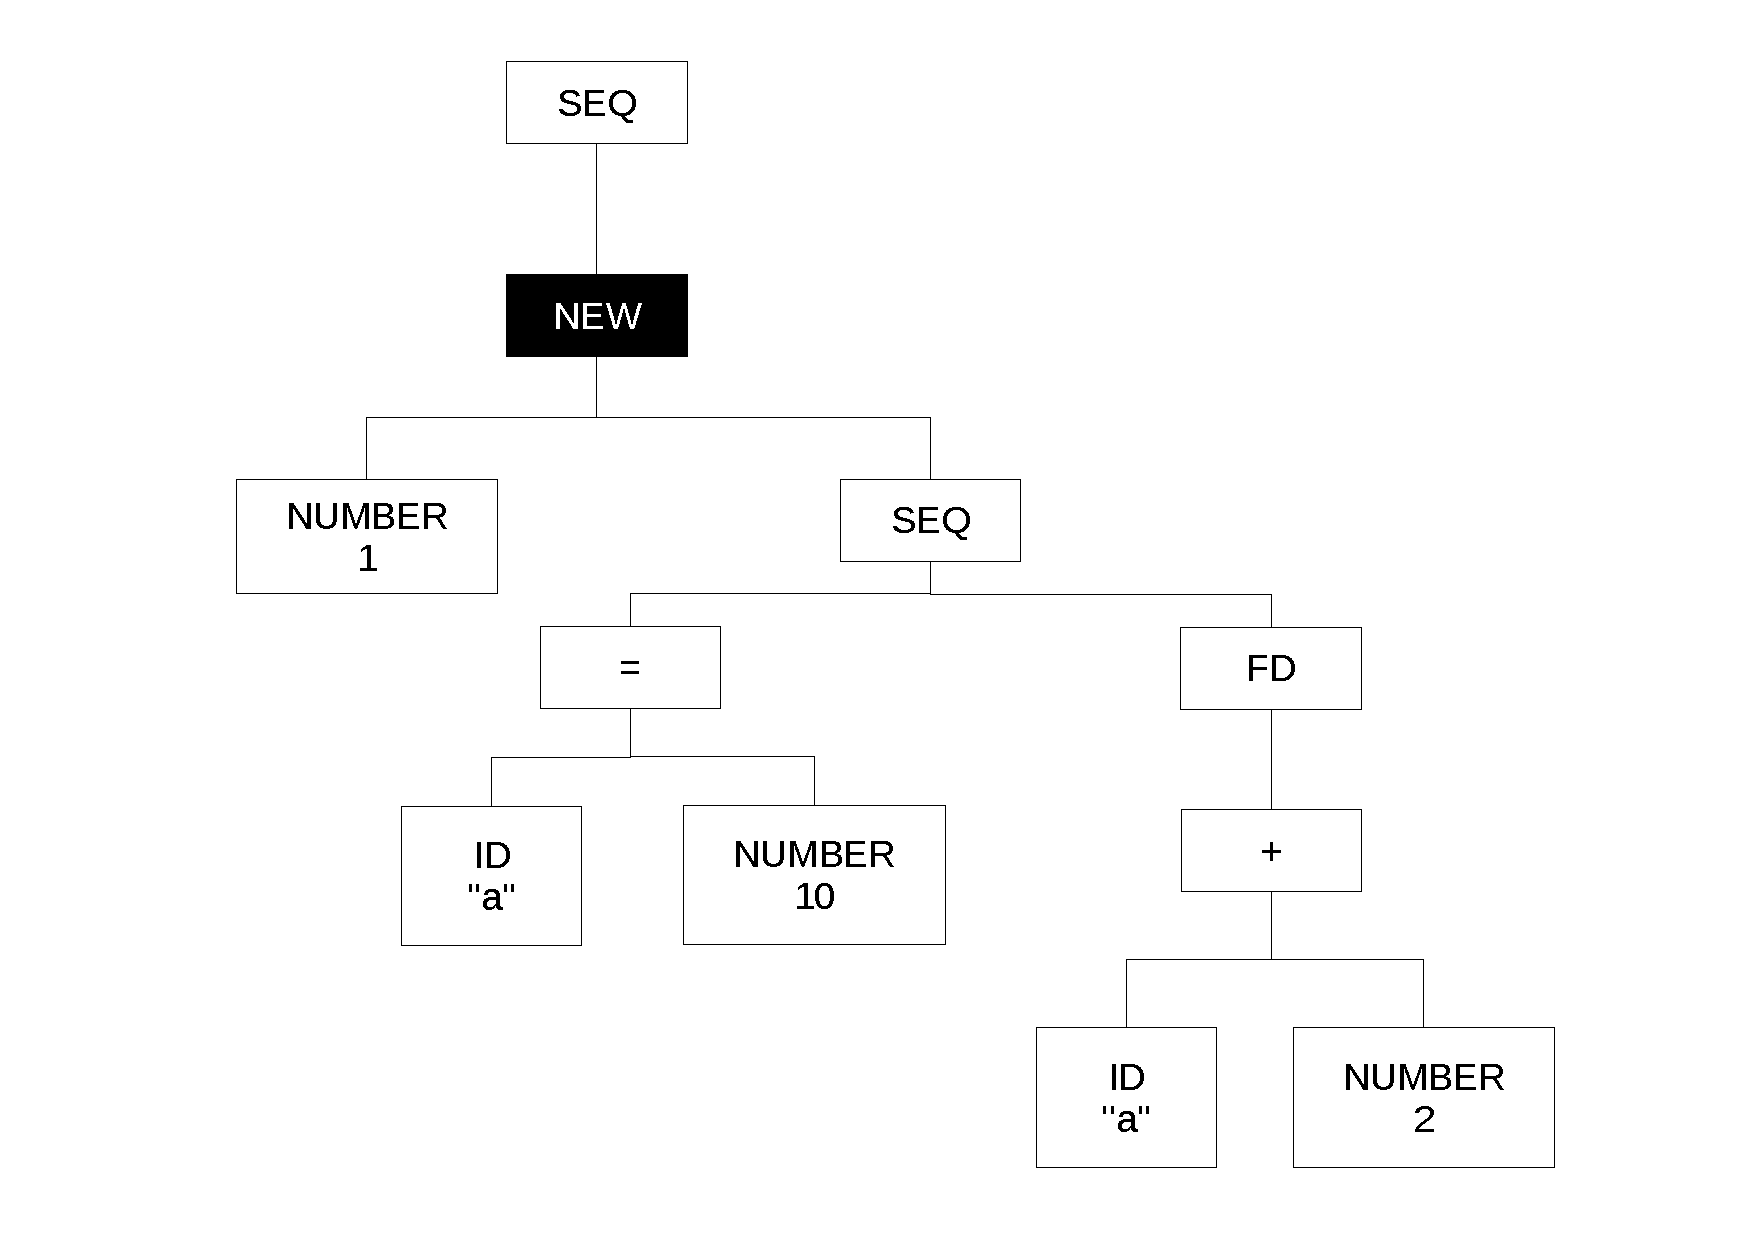
\includegraphics[scale=0.3]{doc/Presentation/img/arbre2.pdf}
\end{frame}

\begin{frame}[fragile]
	\begin{lstlisting}[language=Stibbons]
new agent {
  a = 10
  fd a + 2
}

4 new agent{
  fd 10
}
	\end{lstlisting}
\end{frame}

\begin{frame}
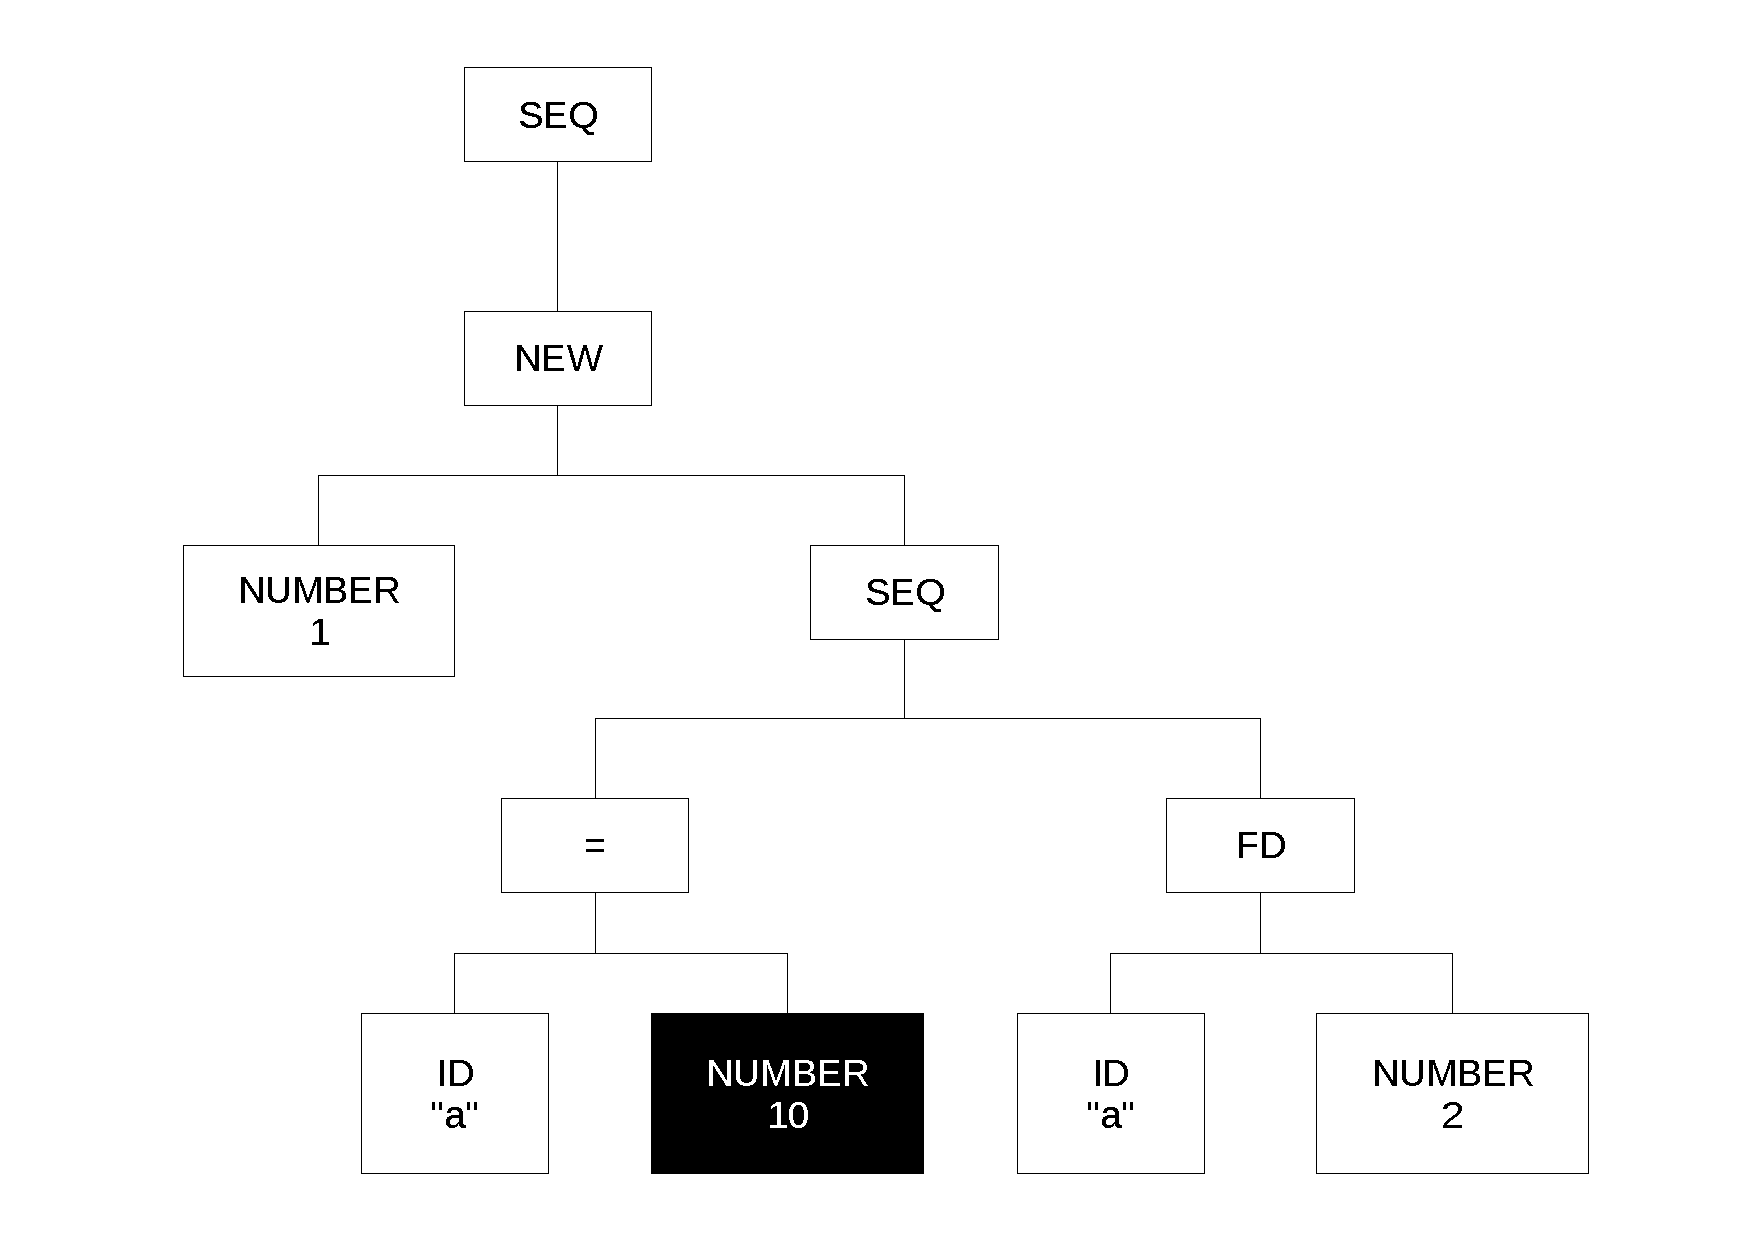
\includegraphics[scale=0.3]{doc/Presentation/img/arbre3.pdf}
\end{frame}

\begin{frame}
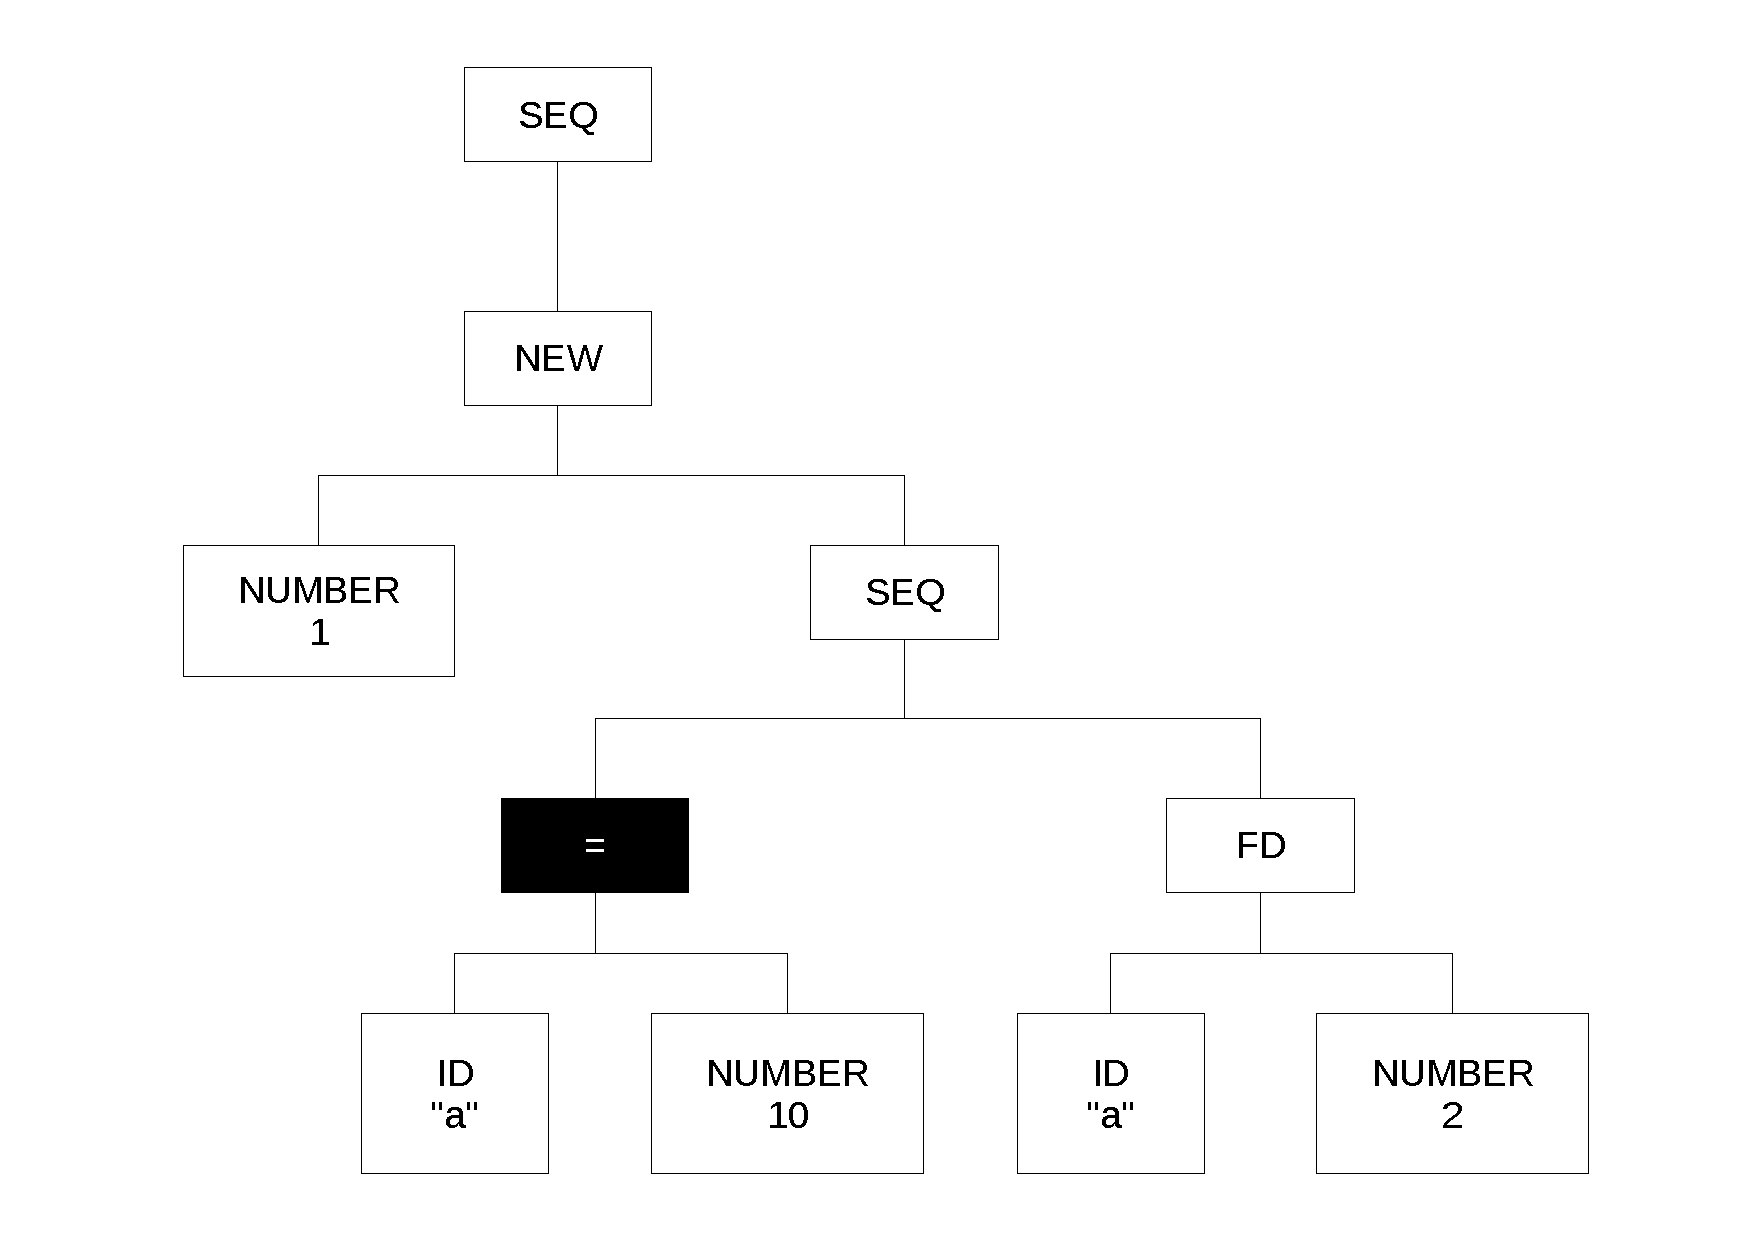
\includegraphics[scale=0.3]{doc/Presentation/img/arbre4.pdf}
\end{frame}

\begin{frame}
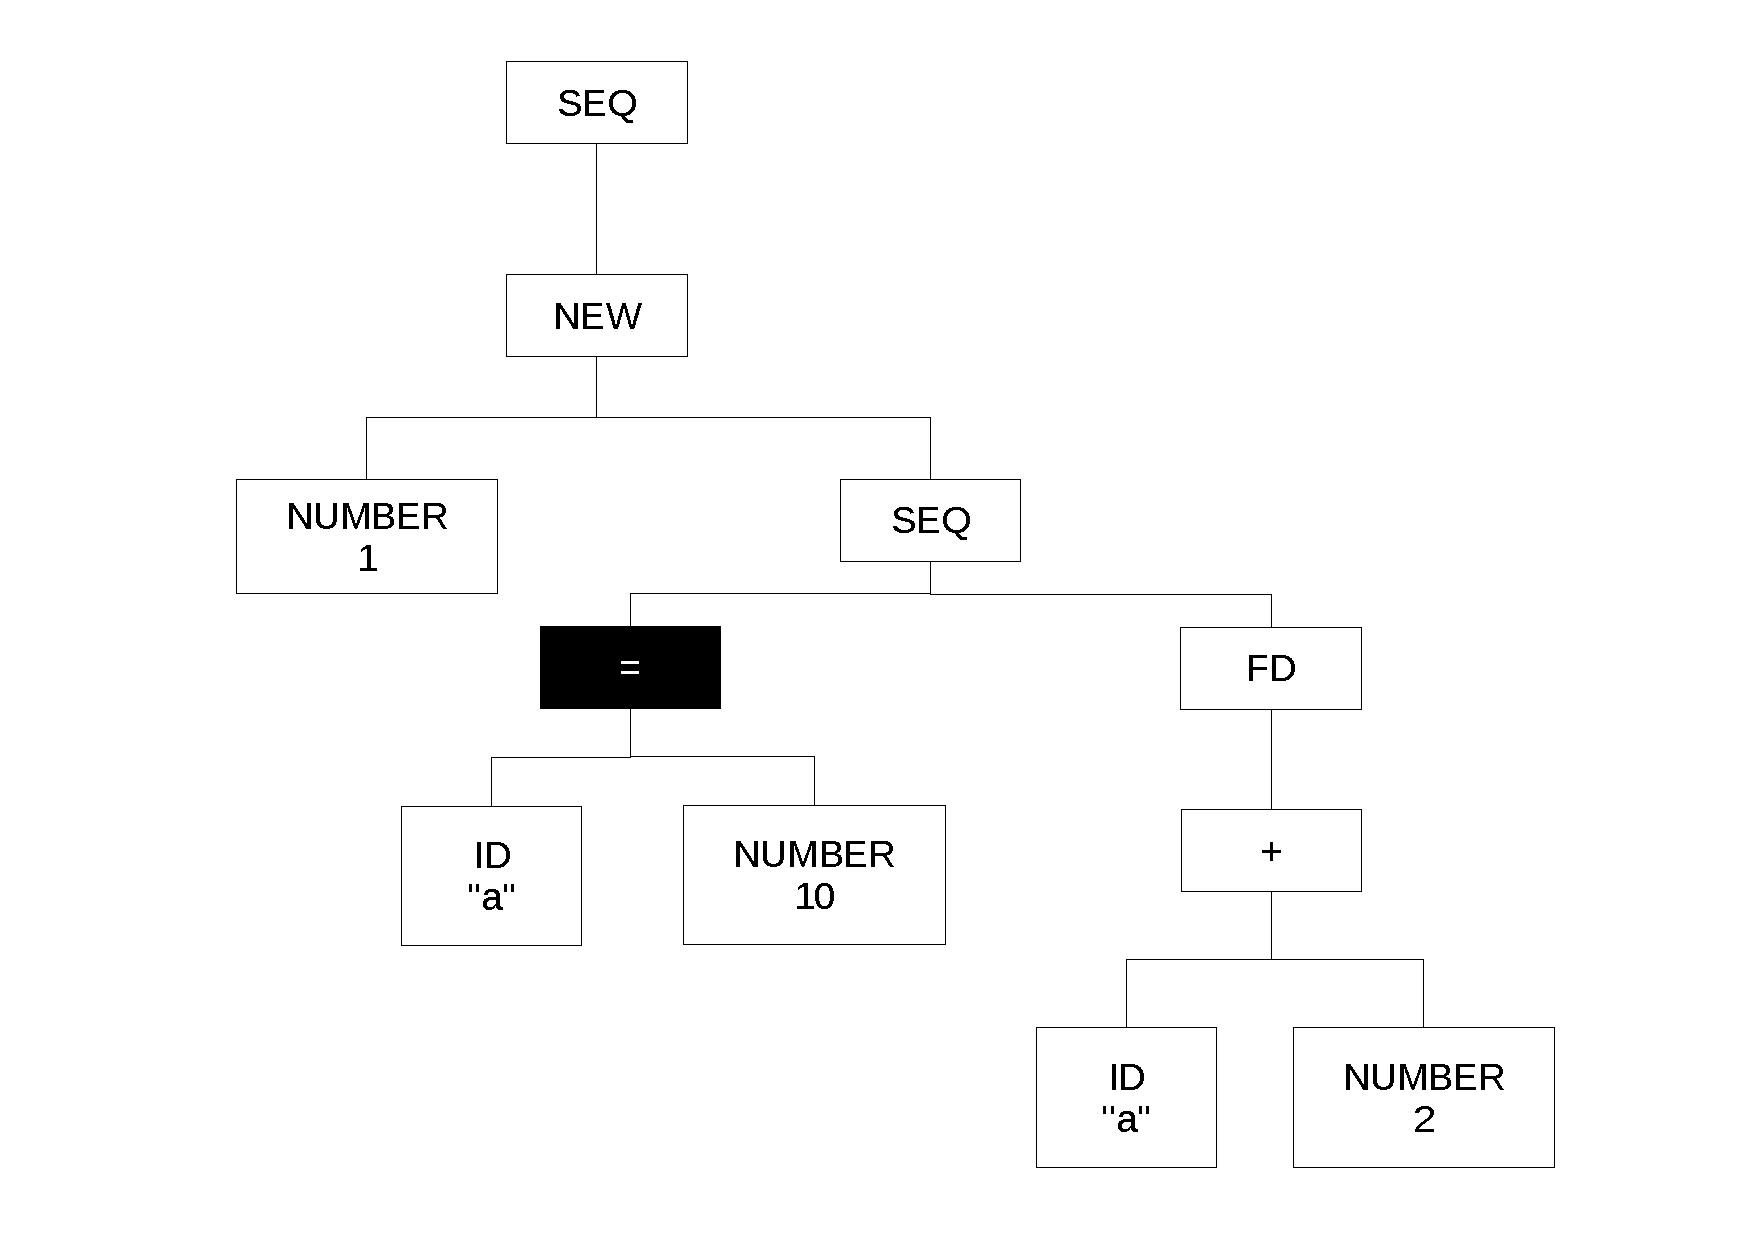
\includegraphics[scale=0.3]{doc/Presentation/img/arbre5.pdf}
\end{frame}

\begin{frame}
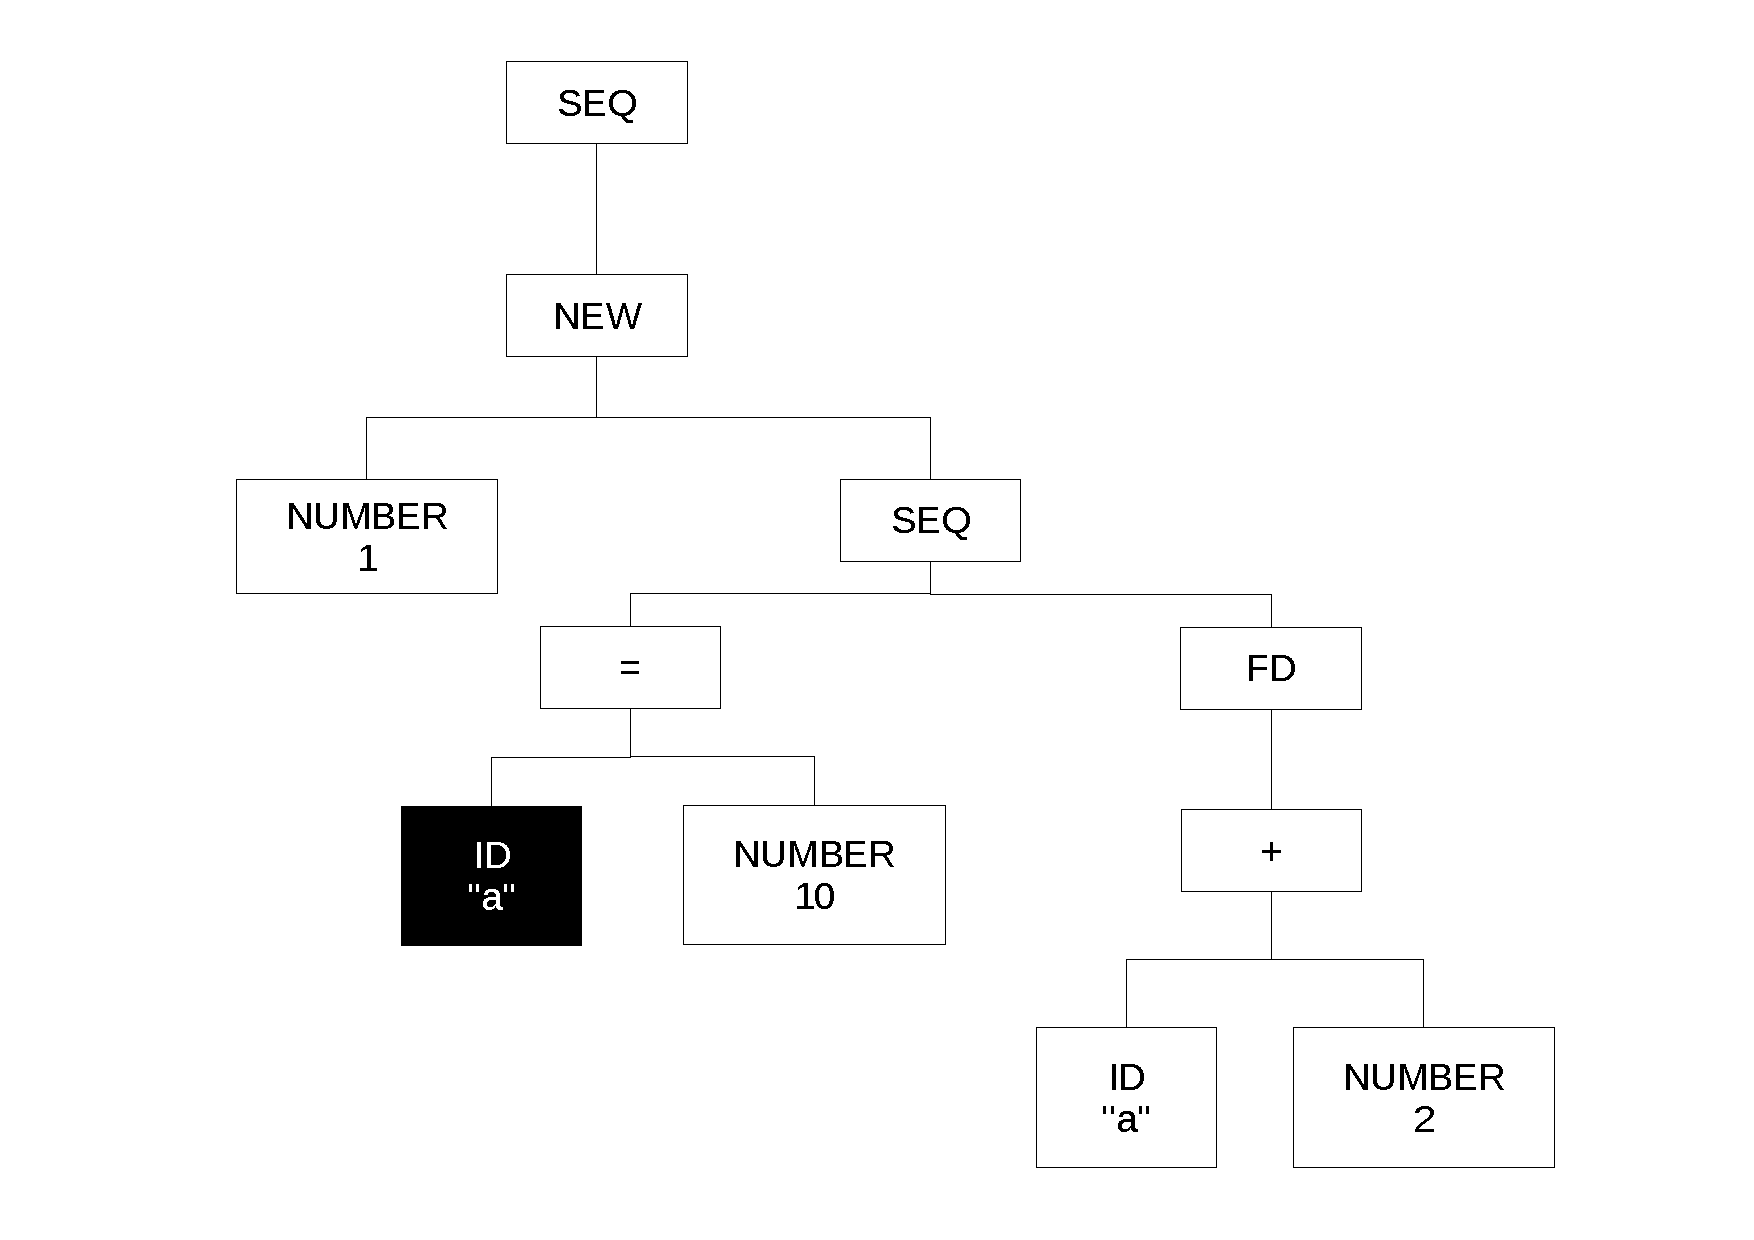
\includegraphics[scale=0.3]{doc/Presentation/img/arbre6.pdf}
\end{frame}

\begin{frame}
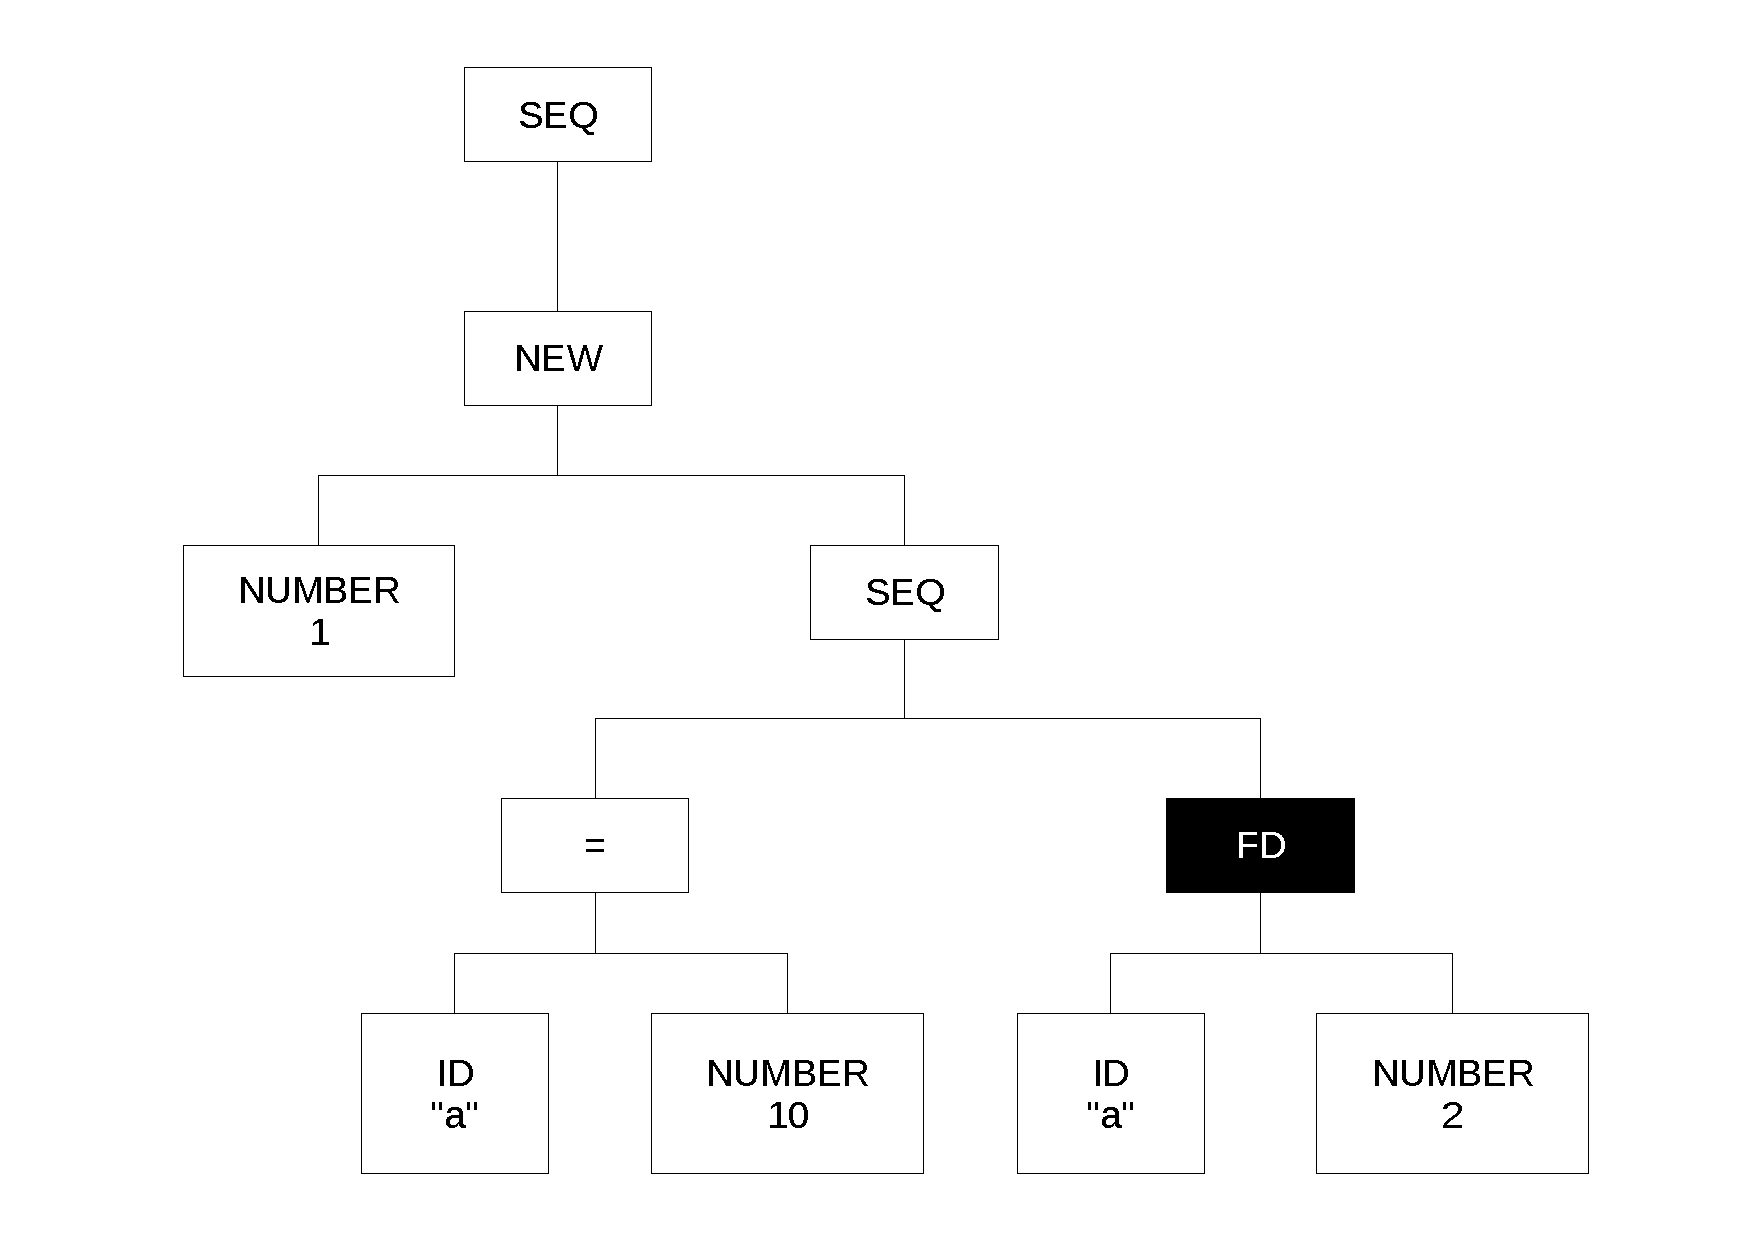
\includegraphics[scale=0.3]{doc/Presentation/img/arbre7.pdf}
\end{frame}

\begin{frame}
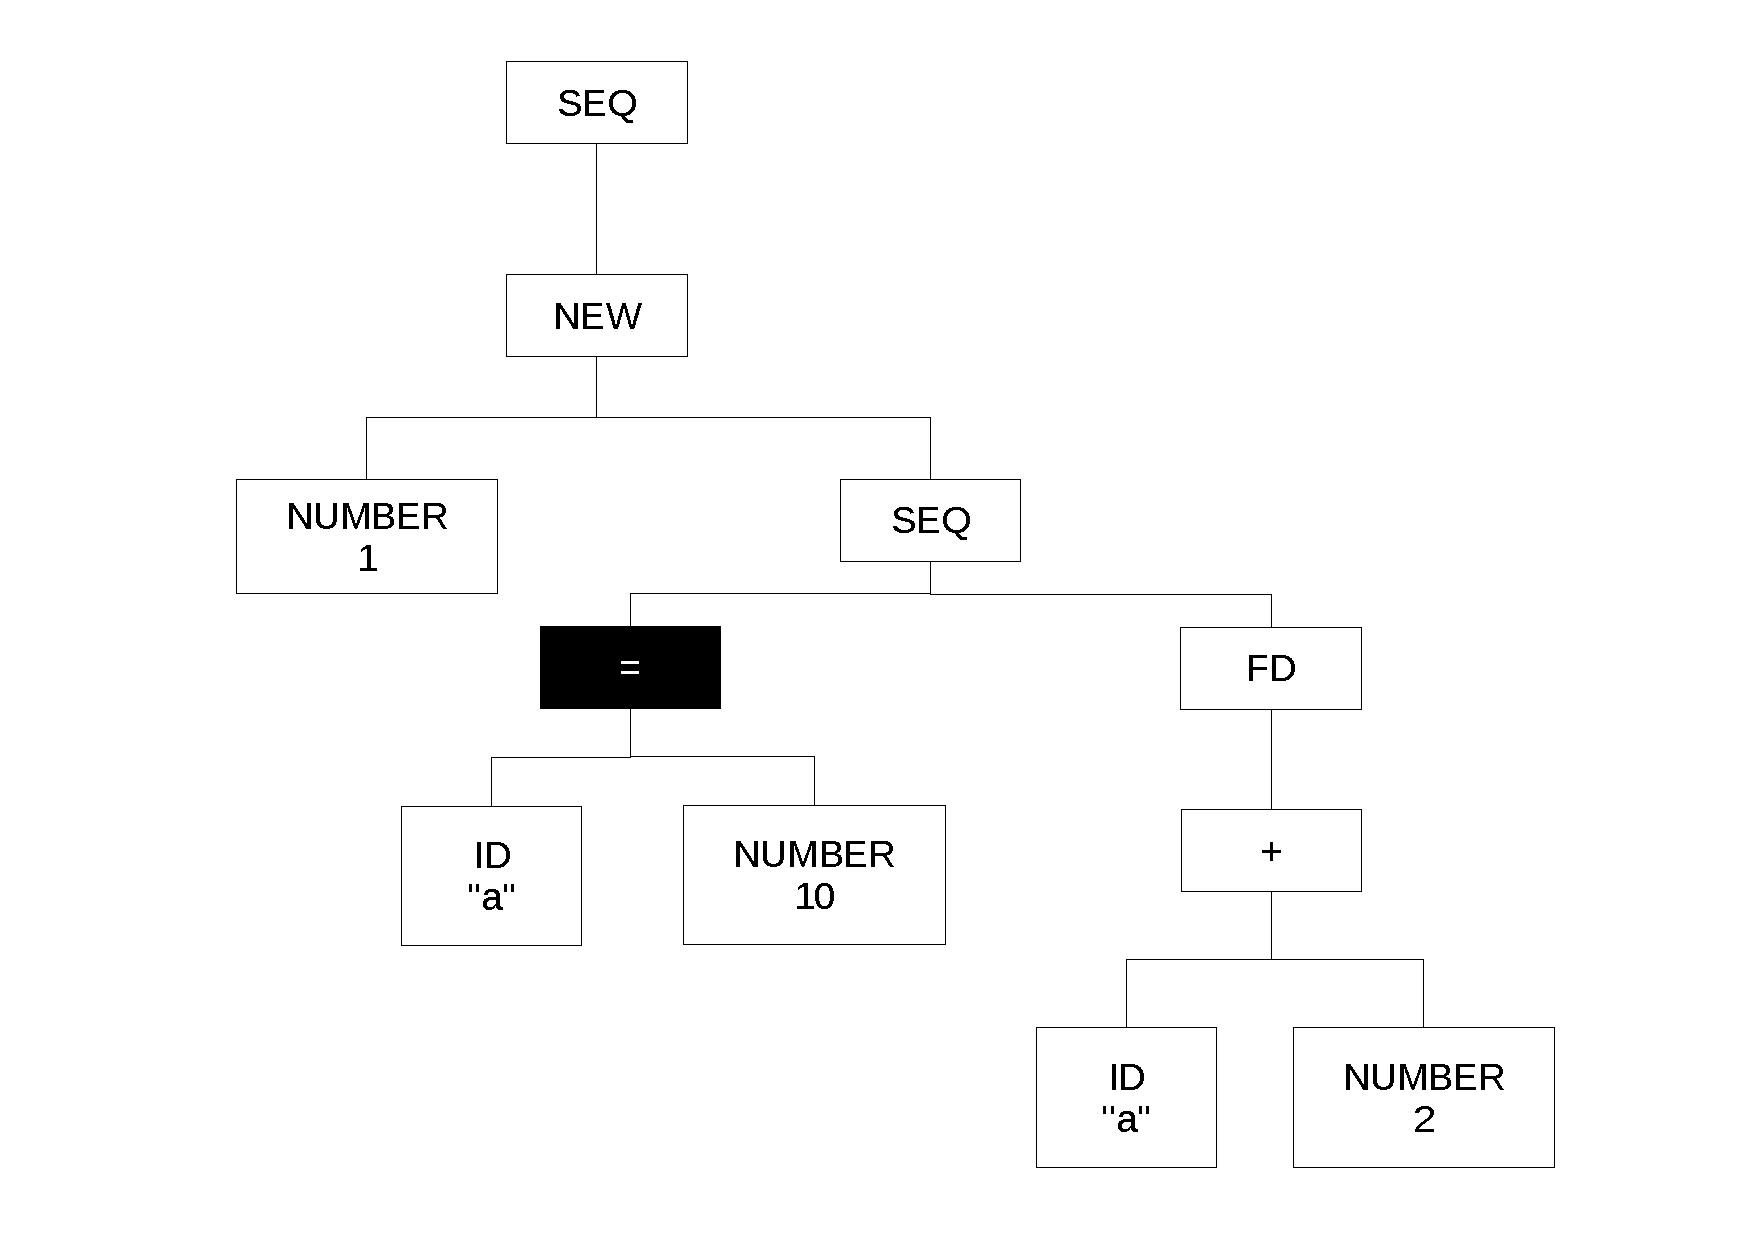
\includegraphics[scale=0.3]{doc/Presentation/img/arbre5.pdf}
\end{frame}

\begin{frame}
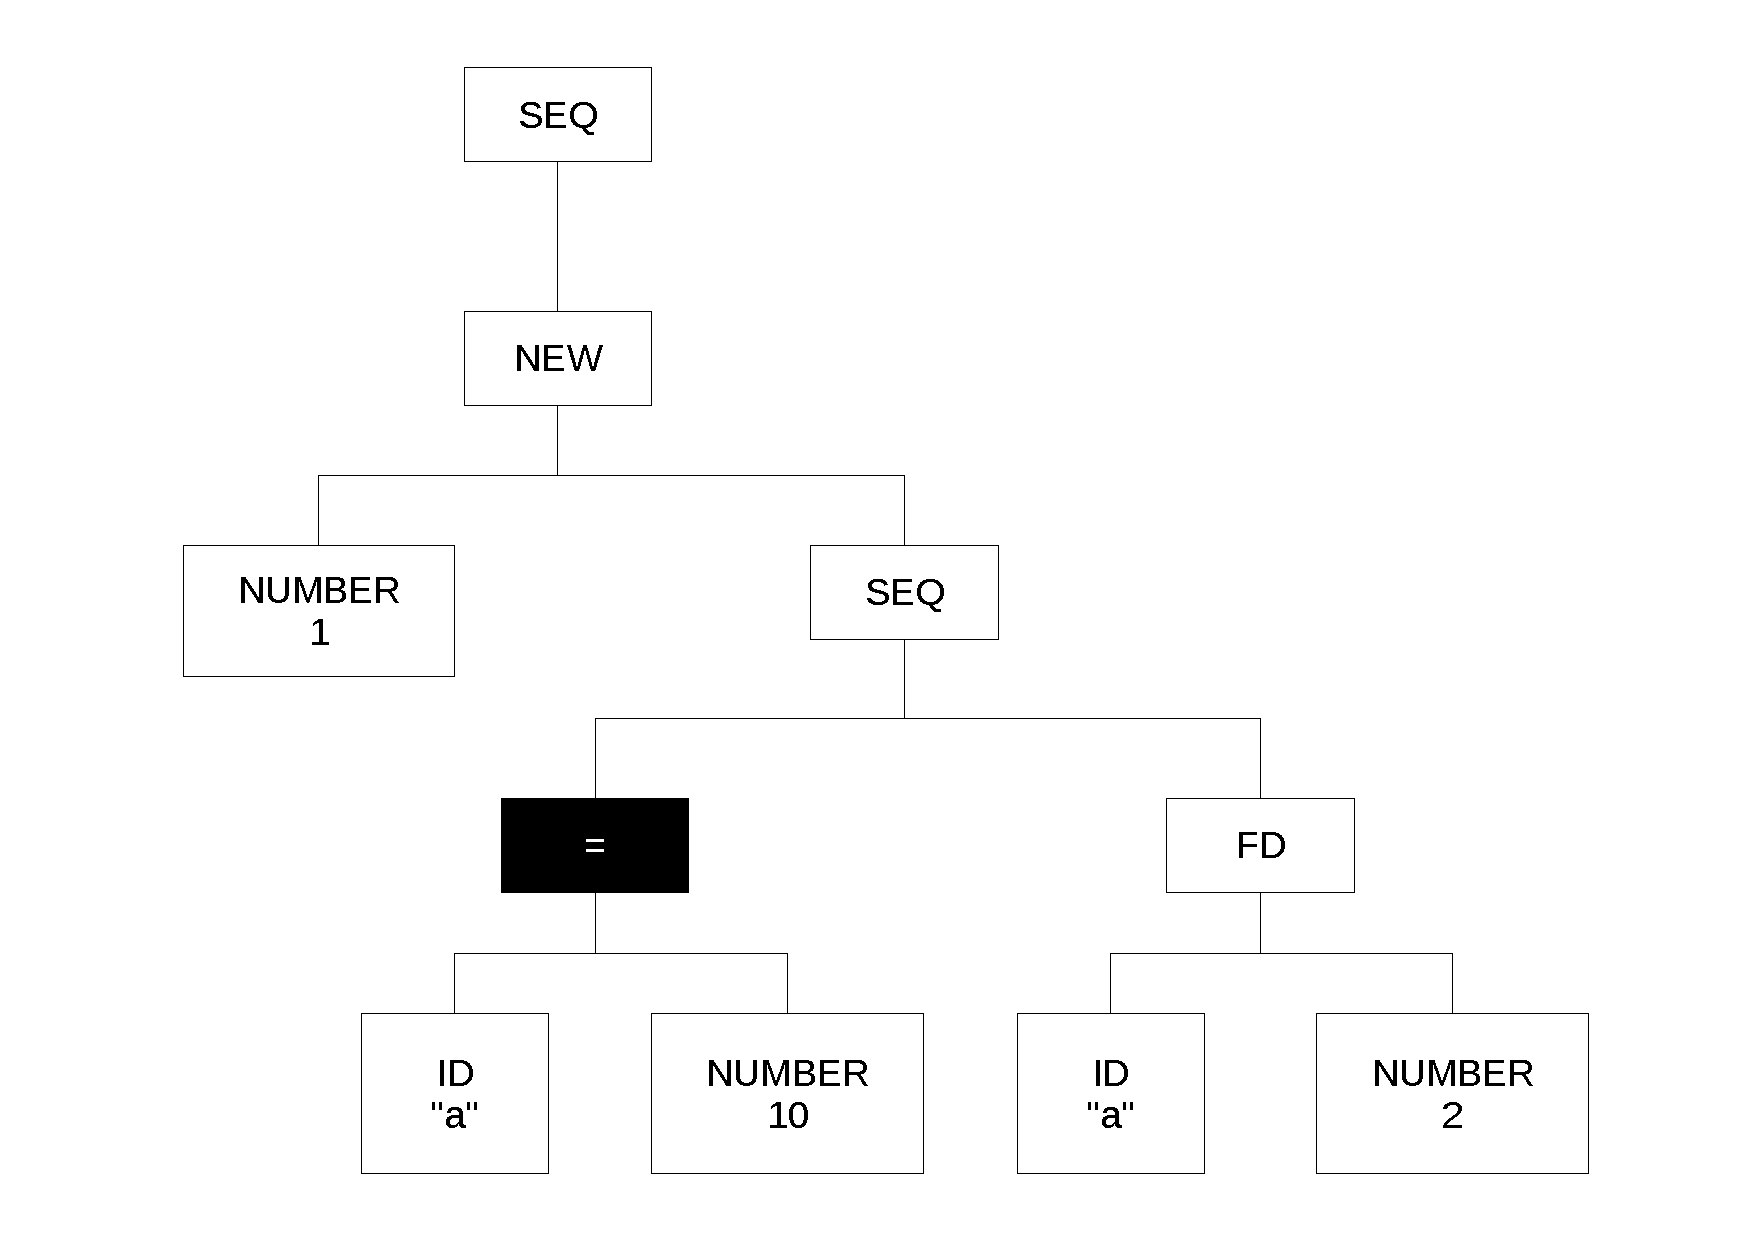
\includegraphics[scale=0.3]{doc/Presentation/img/arbre4.pdf}
\end{frame}

\begin{frame}
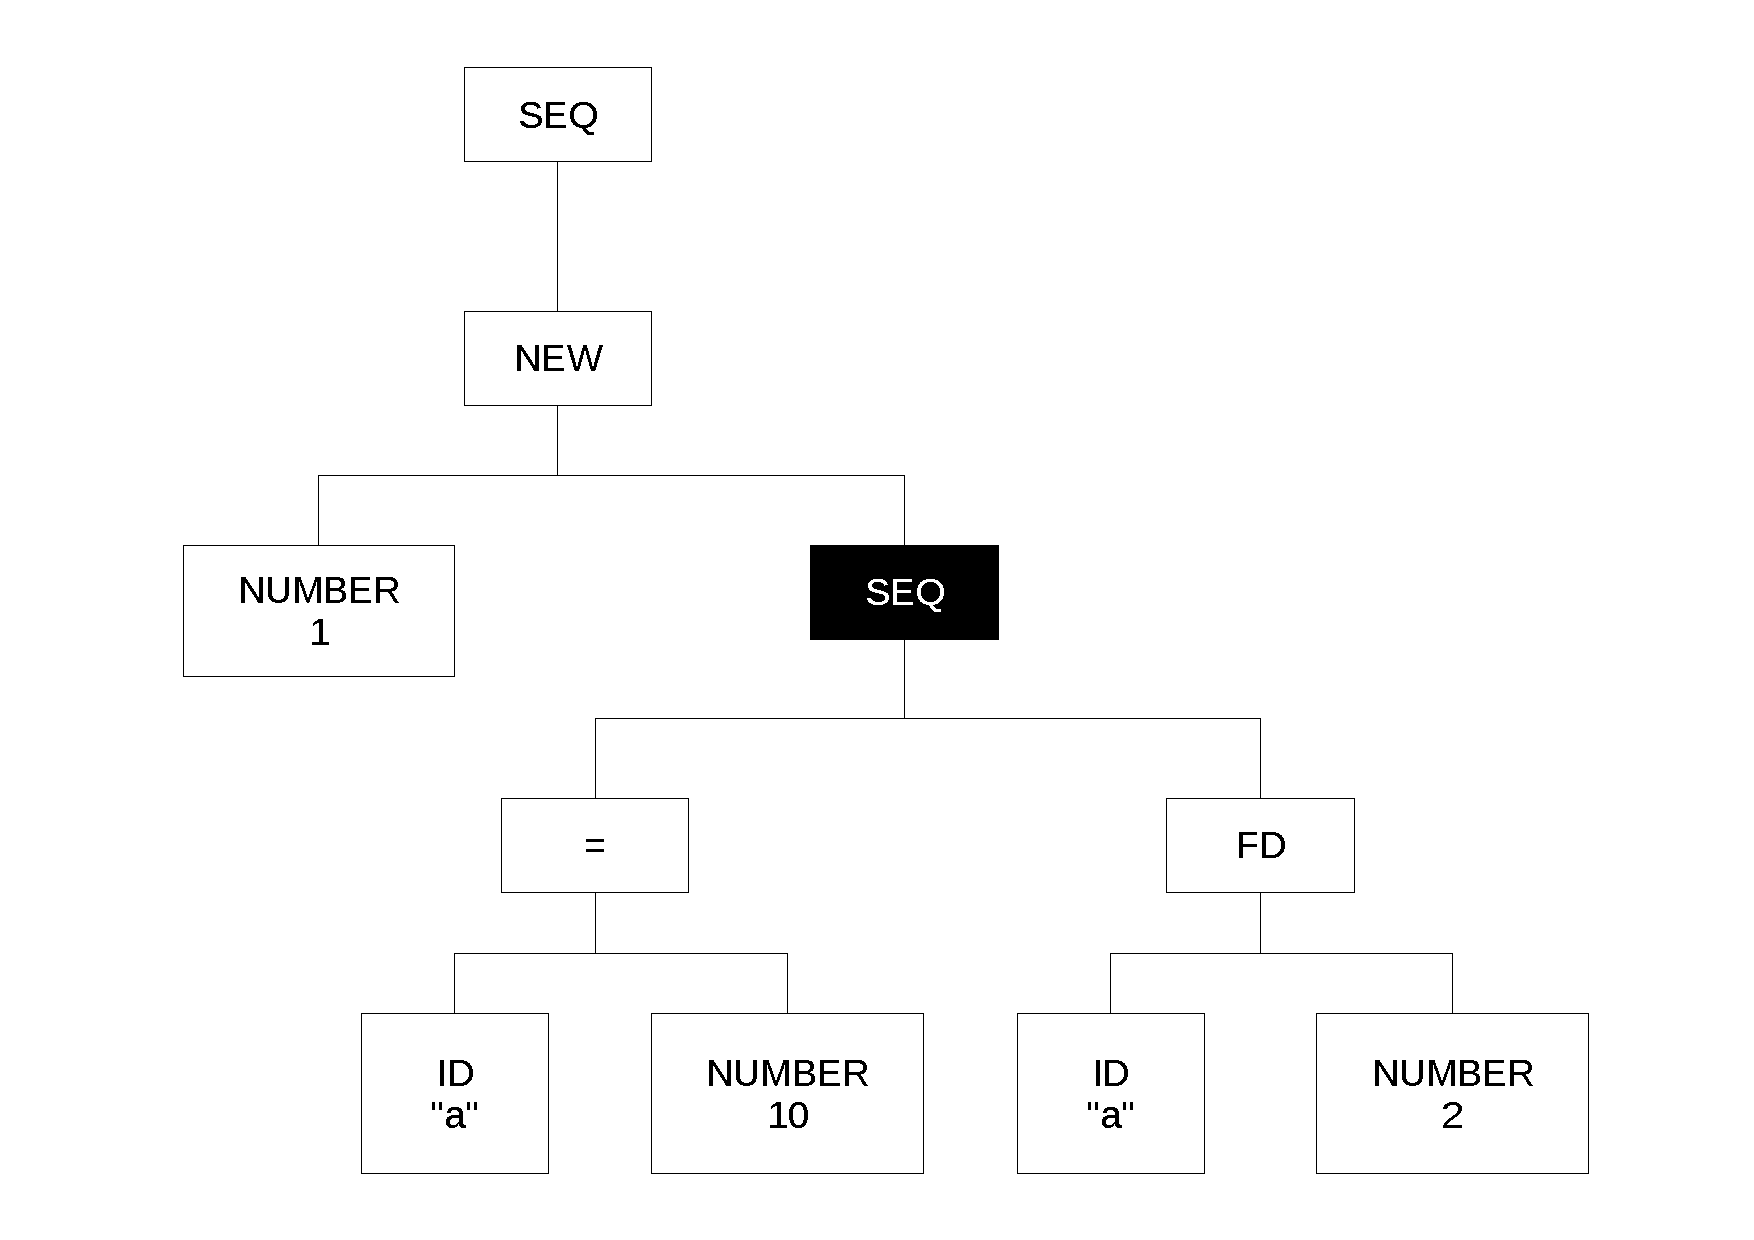
\includegraphics[scale=0.3]{doc/Presentation/img/arbre8.pdf}
\end{frame}

\begin{frame}
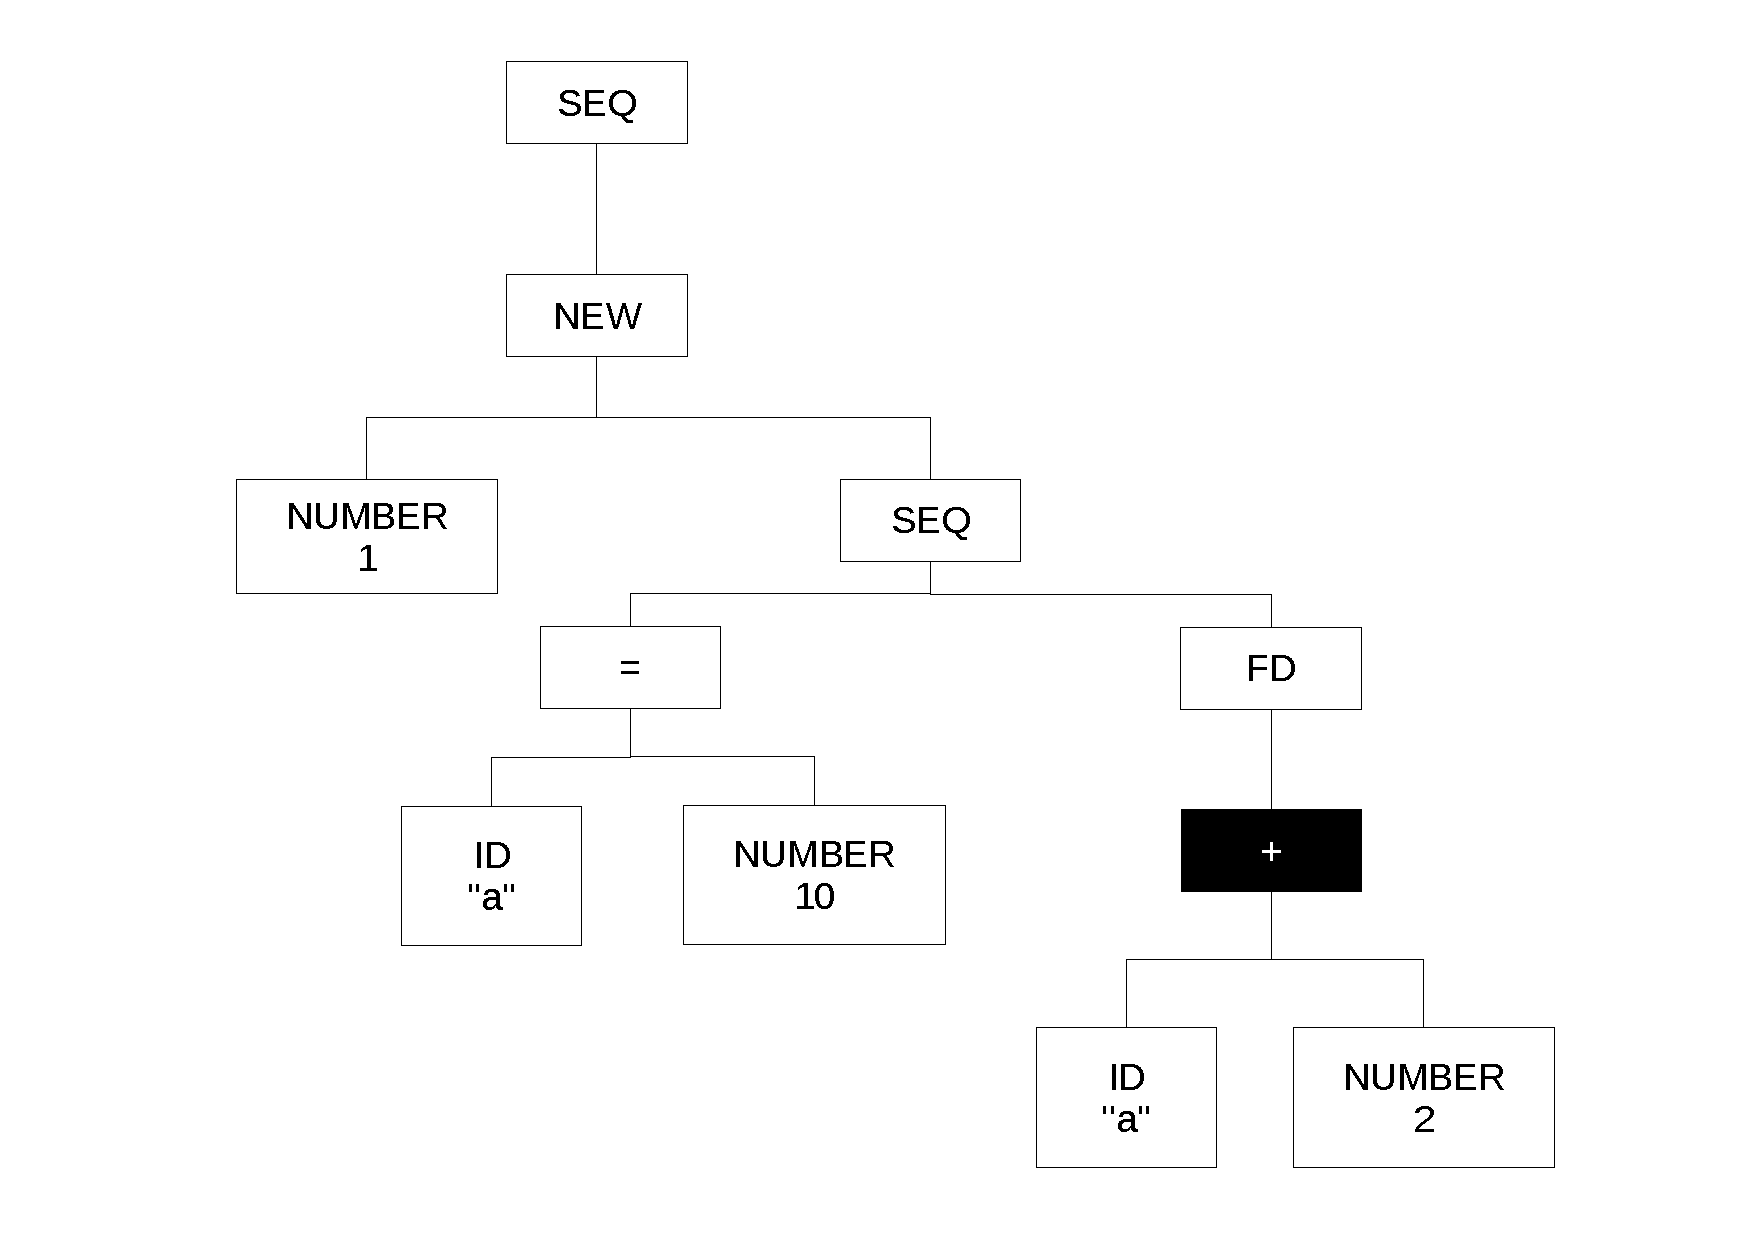
\includegraphics[scale=0.3]{doc/Presentation/img/arbre9.pdf}
\end{frame}

\begin{frame}
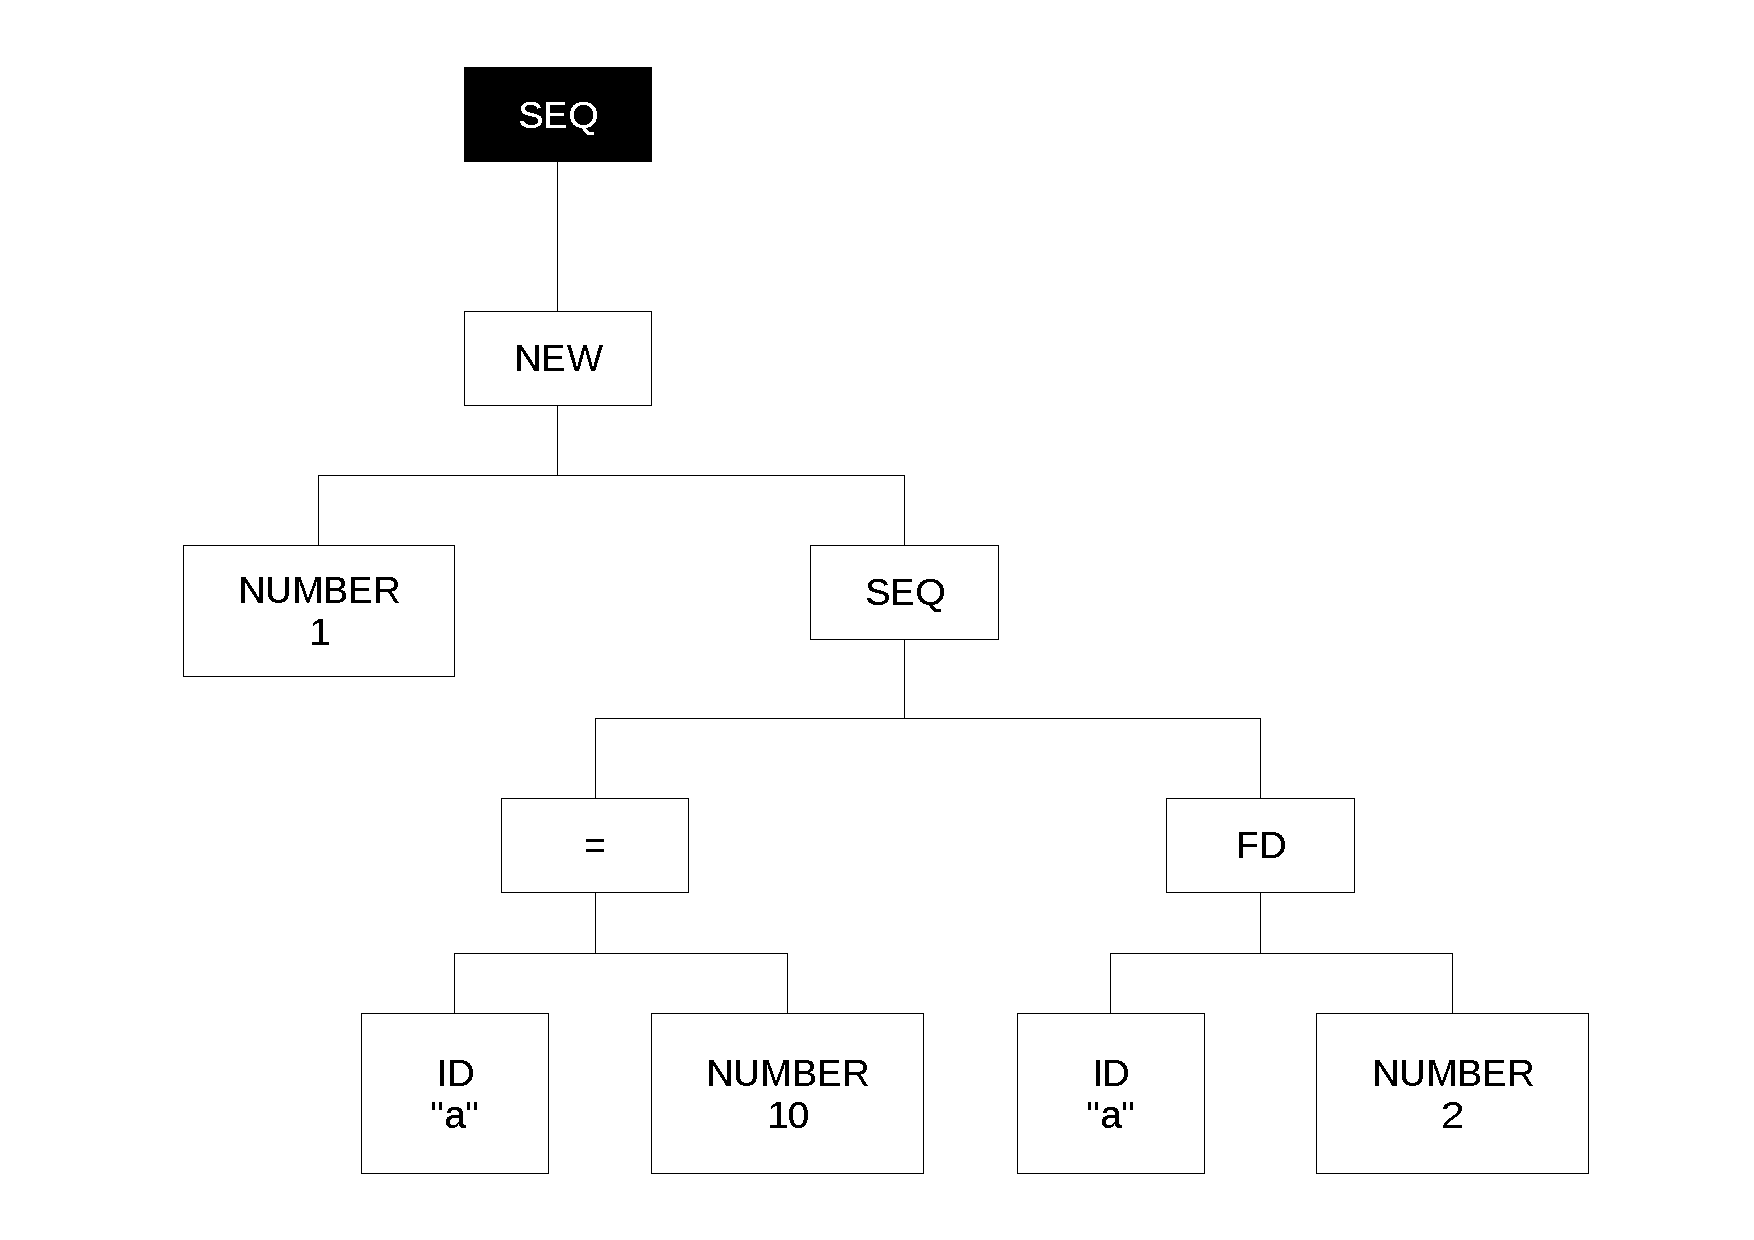
\includegraphics[scale=0.3]{doc/Presentation/img/arbre10.pdf}
\end{frame}

\begin{frame}
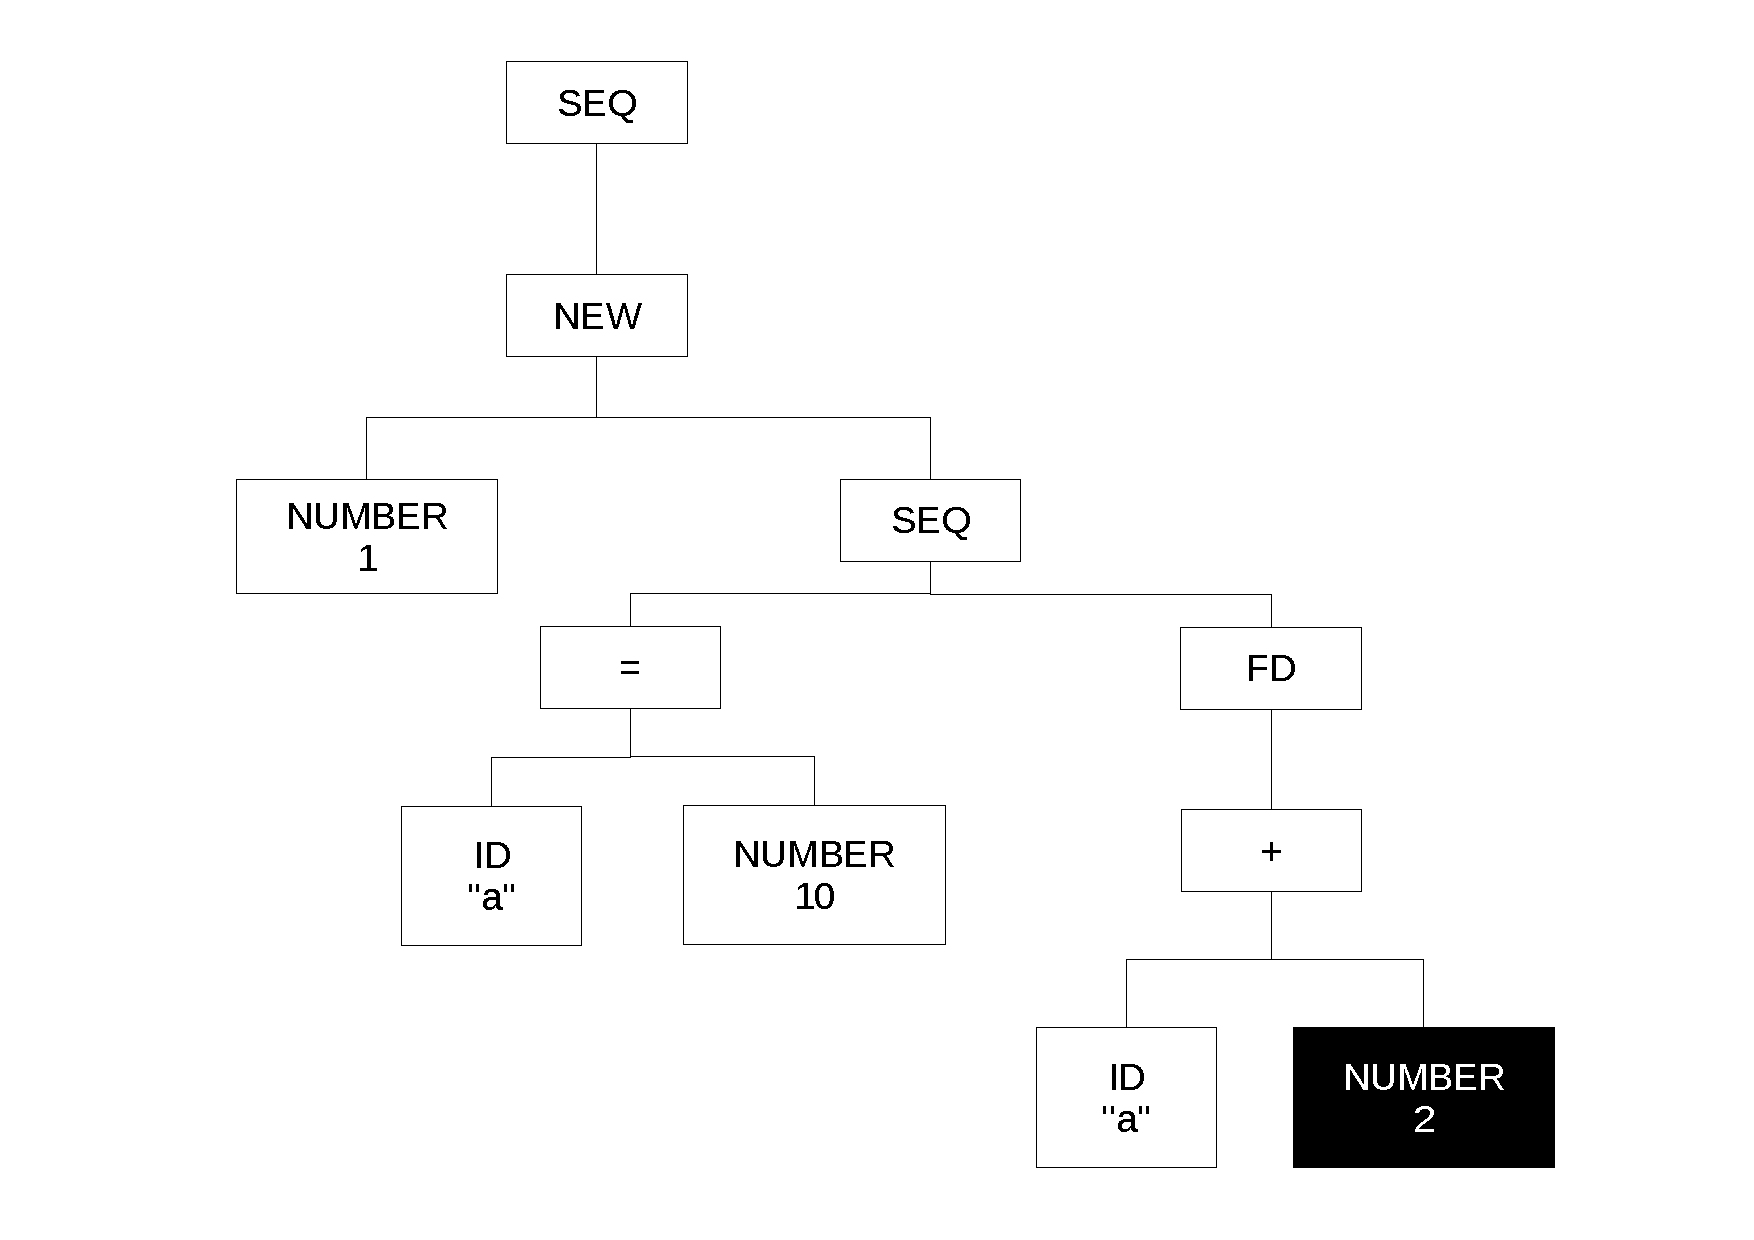
\includegraphics[scale=0.3]{doc/Presentation/img/arbre11.pdf}
\end{frame}

\begin{frame}
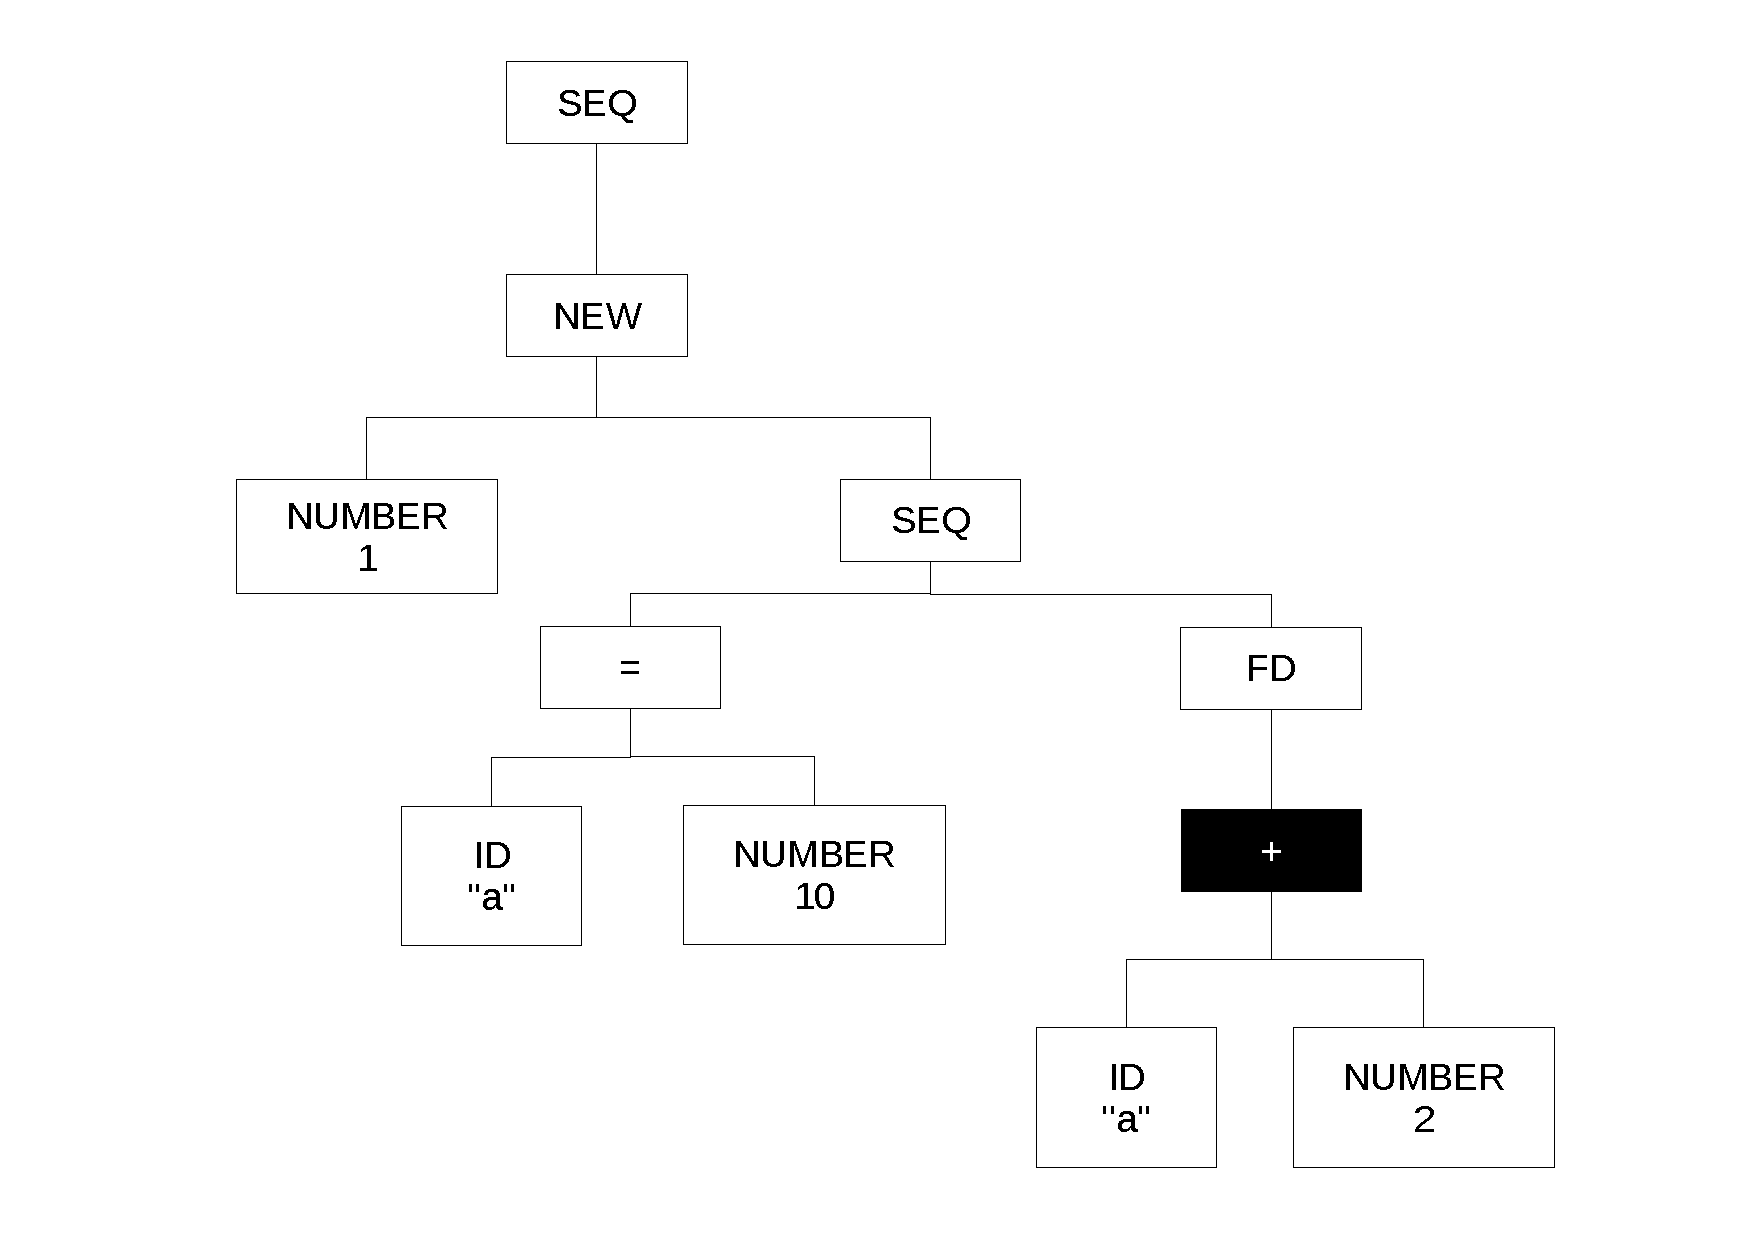
\includegraphics[scale=0.3]{doc/Presentation/img/arbre9.pdf}
\end{frame}

\begin{frame}
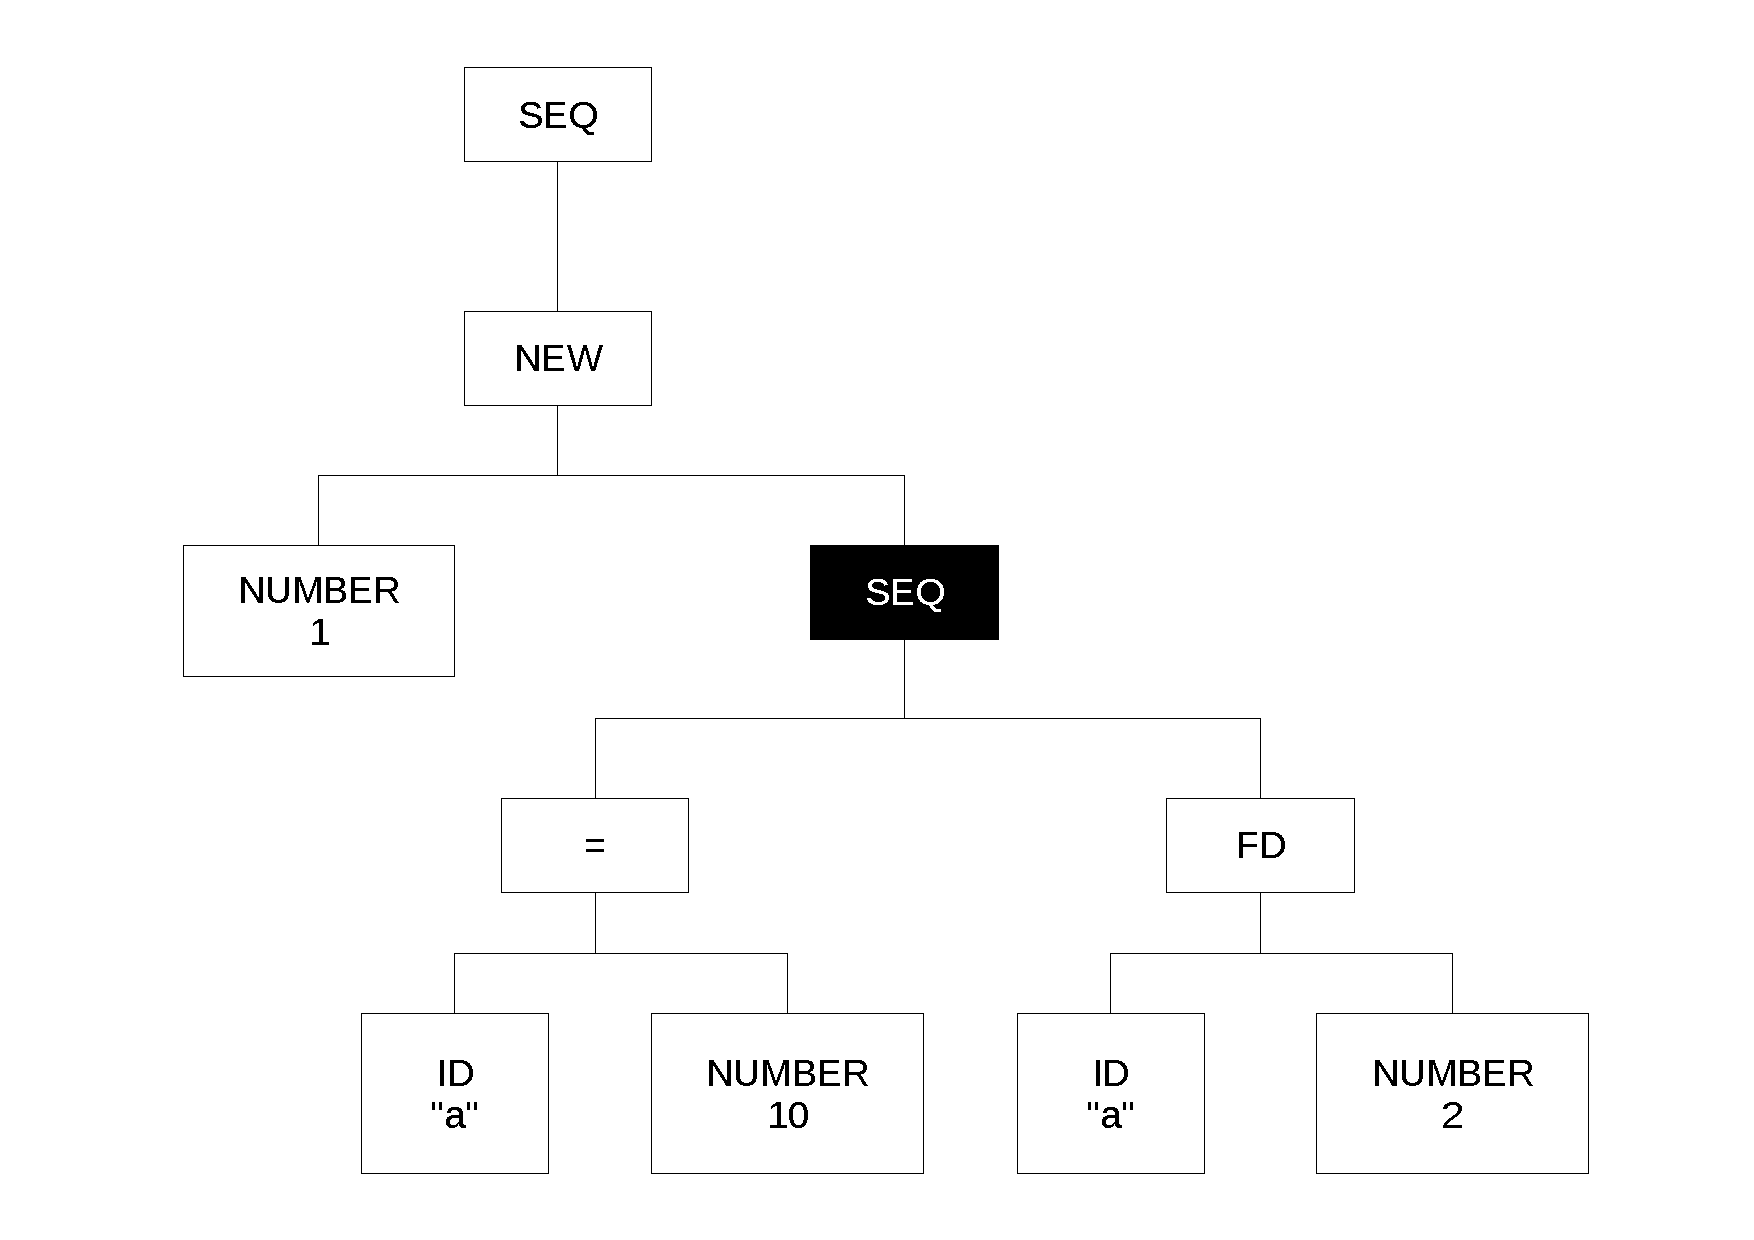
\includegraphics[scale=0.3]{doc/Presentation/img/arbre8.pdf}
\end{frame}

\begin{frame}
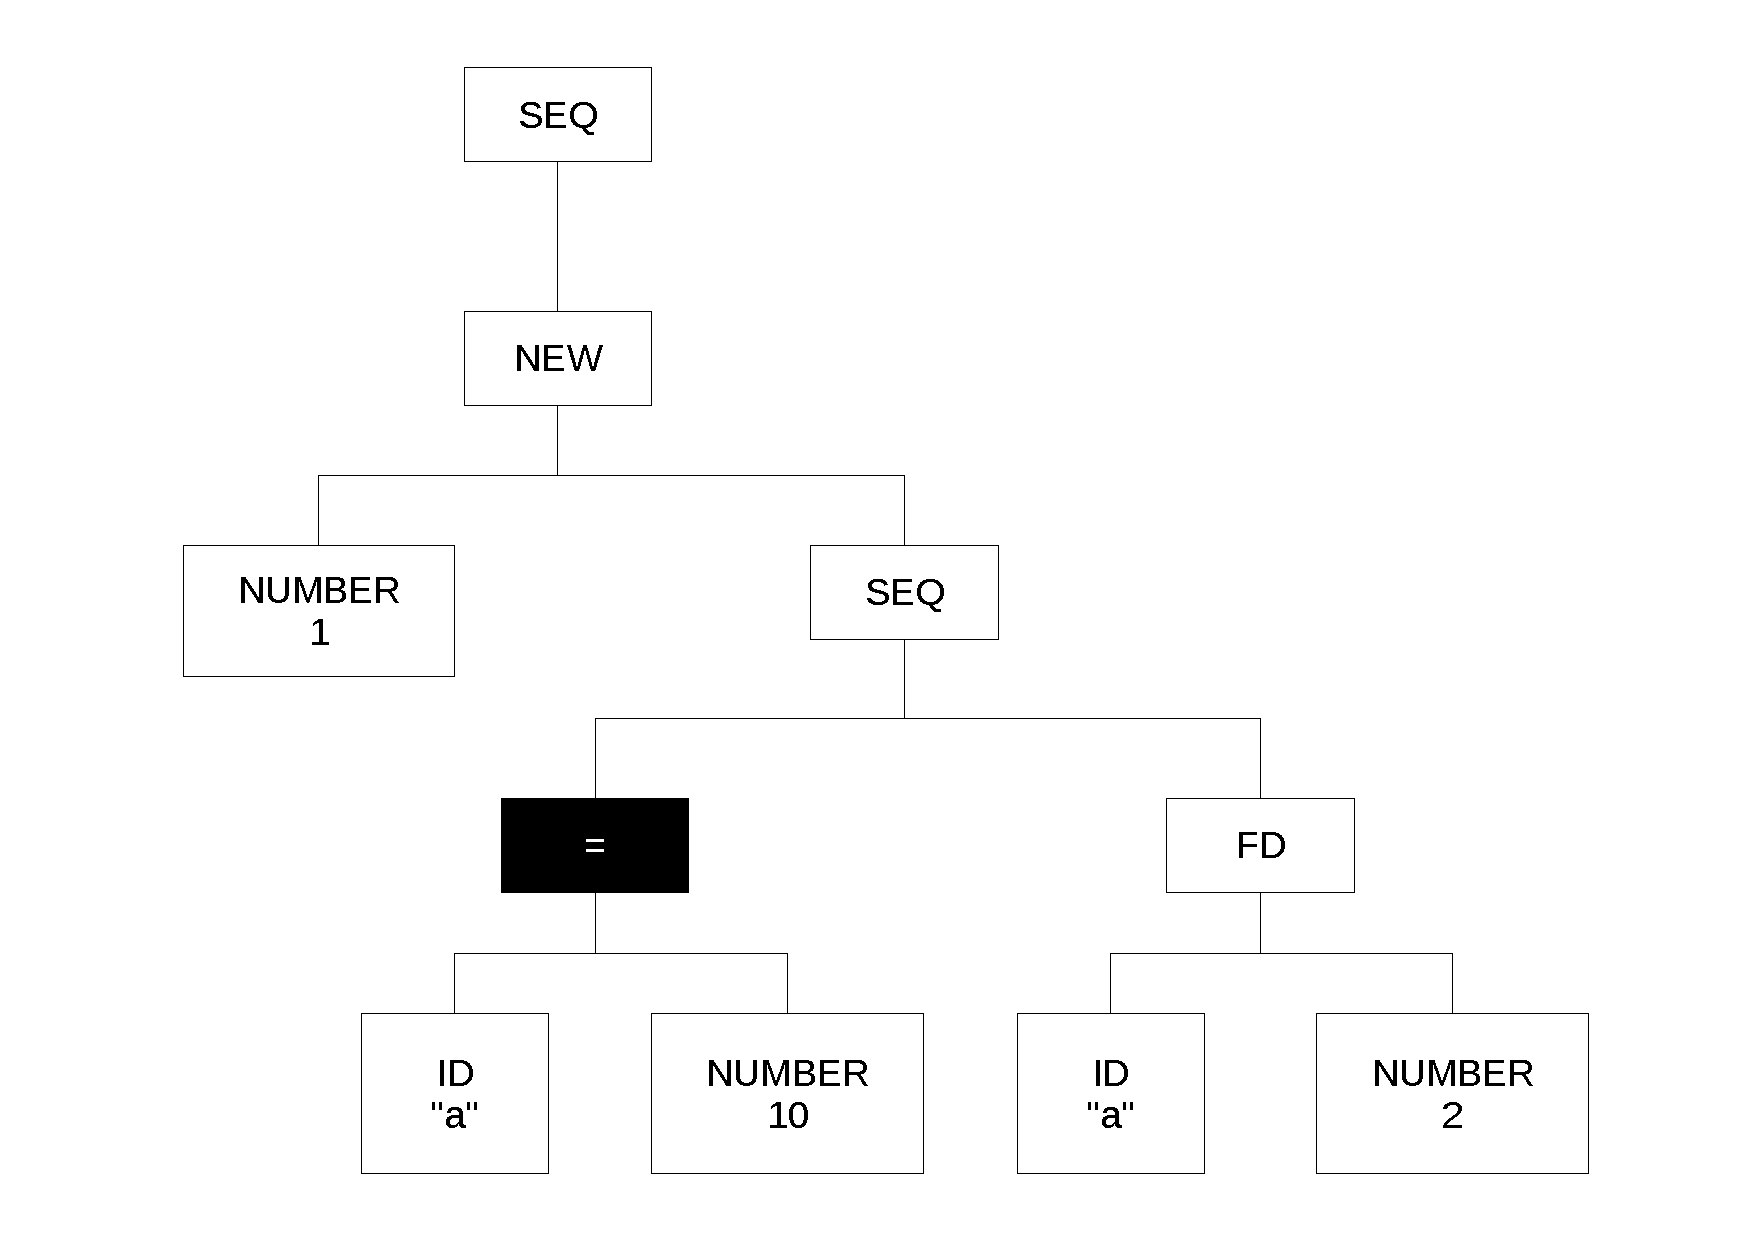
\includegraphics[scale=0.3]{doc/Presentation/img/arbre4.pdf}
\end{frame}

\begin{frame}
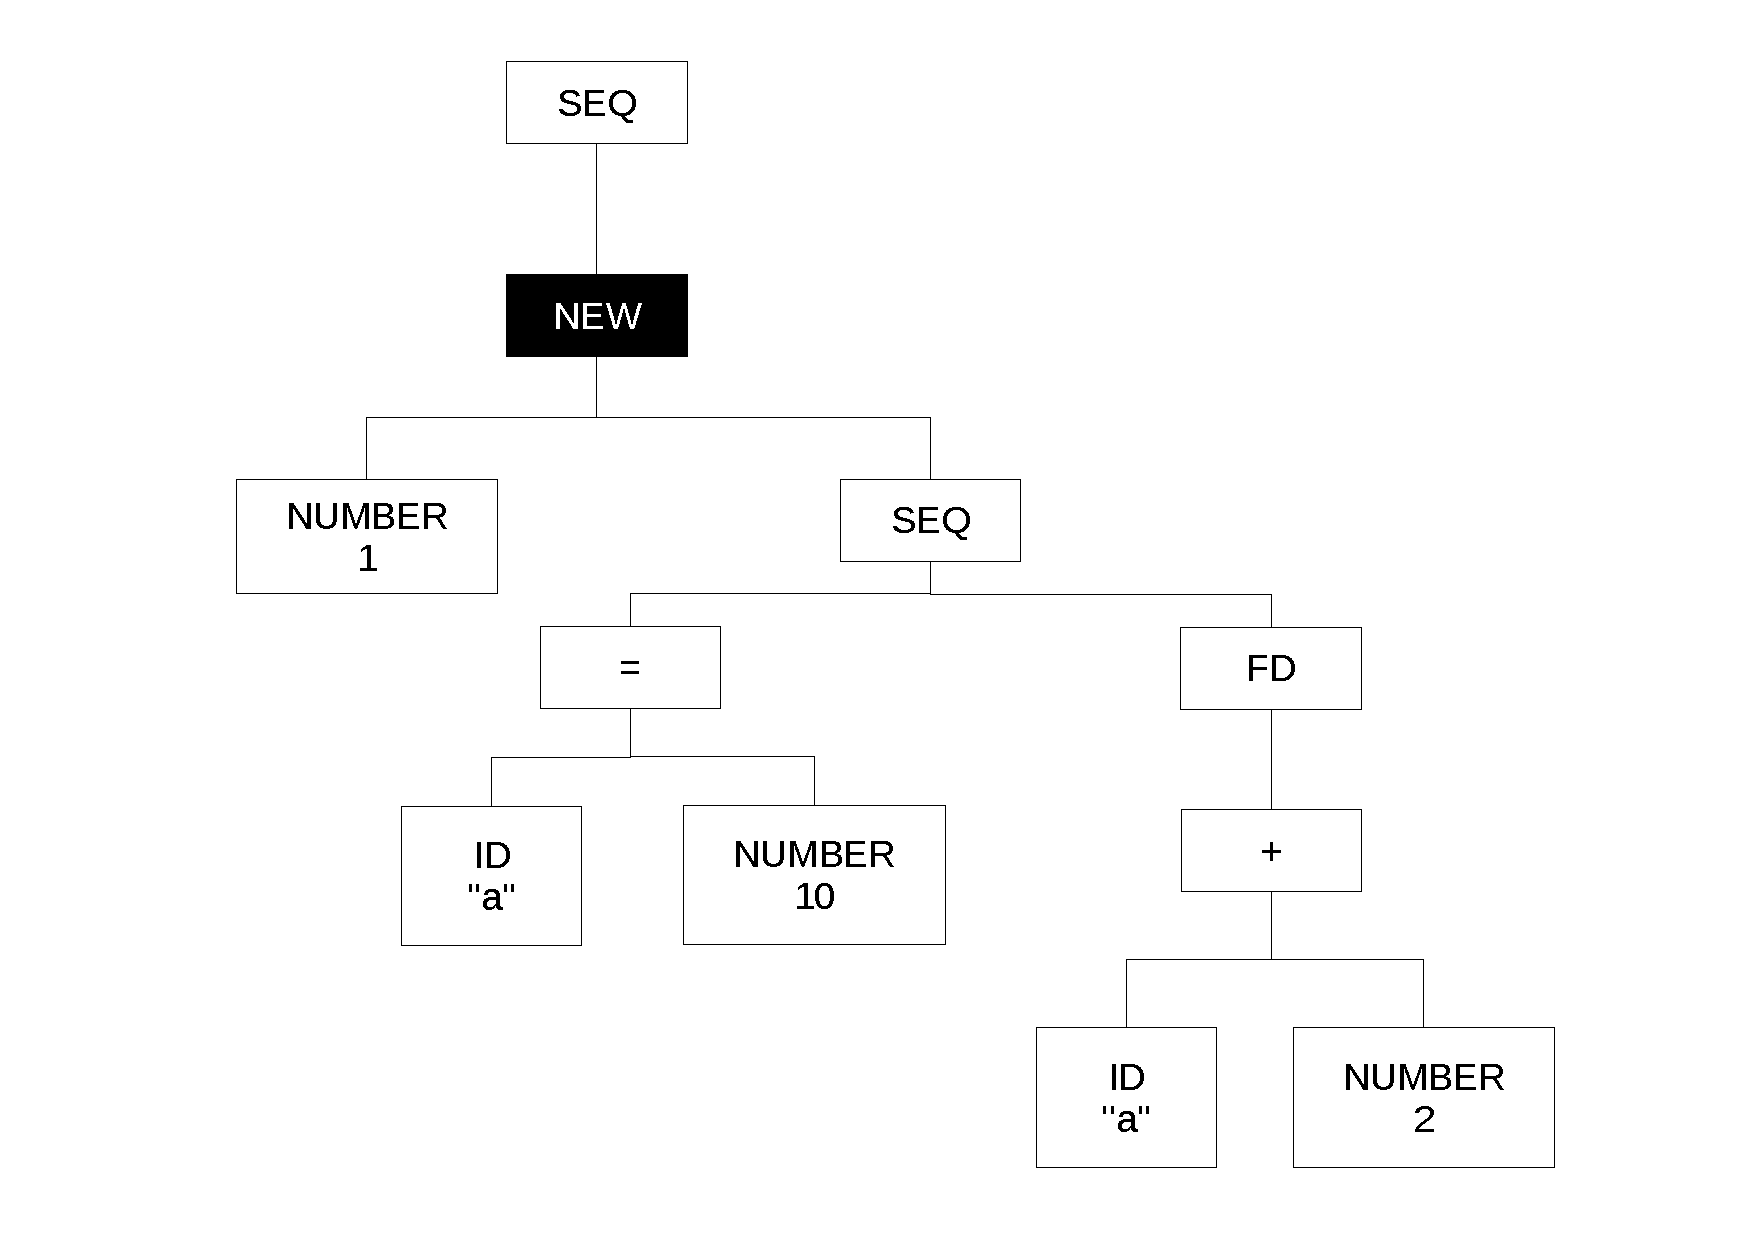
\includegraphics[scale=0.3]{doc/Presentation/img/arbre2.pdf}
\end{frame}

\begin{frame}
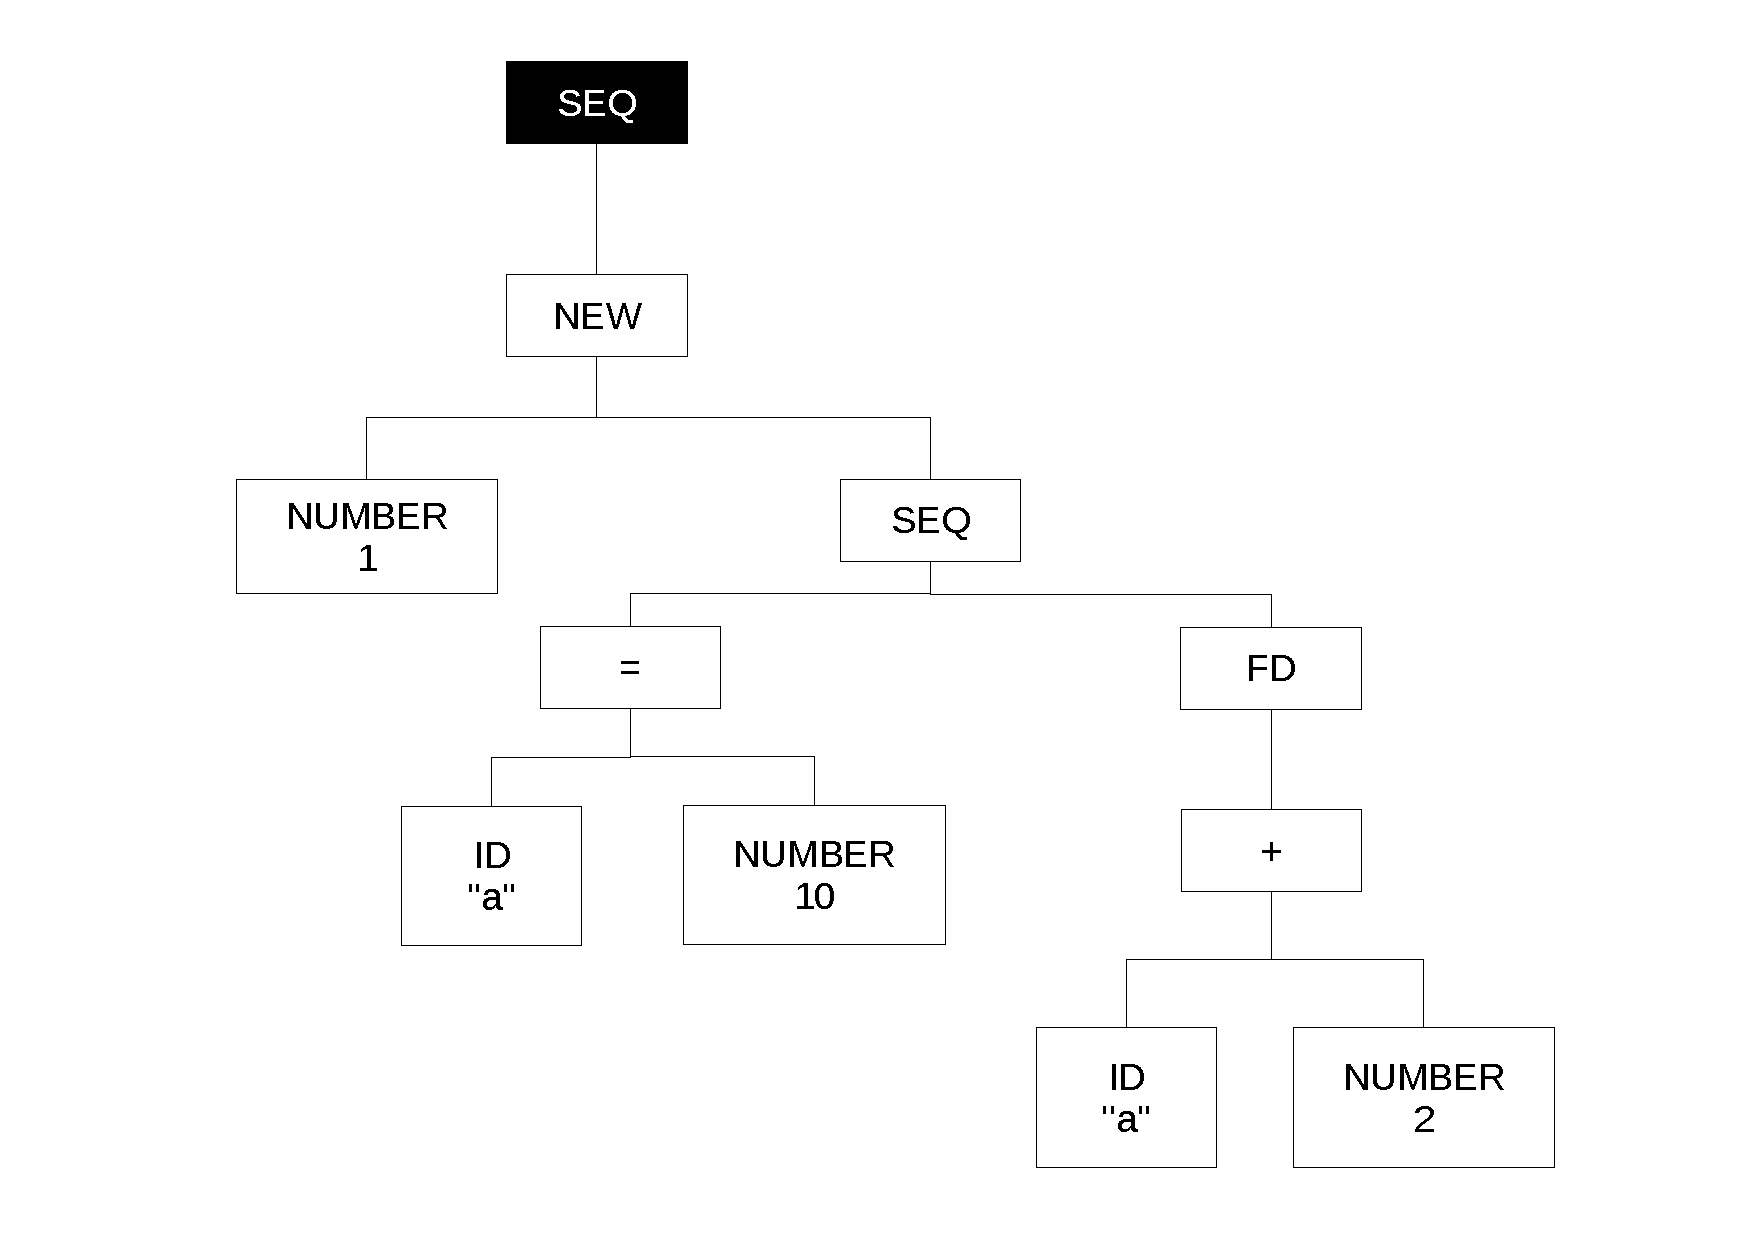
\includegraphics[scale=0.3]{doc/Presentation/img/arbre1.pdf}
\end{frame}

\begin{frame}
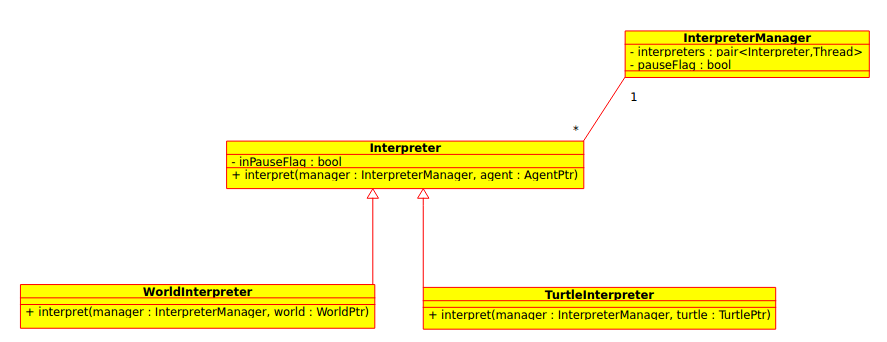
\includegraphics[scale=0.3]{doc/report/uml/interpreterUML.png}
\end{frame}

\begin{frame}
Rôle de l'interprète manager~:
\begin{itemize}
	\item Alerter des éventuelles pauses~;
	\item Création d'un monde avec les directives choisies~;
	\item Gérer les interpréteurs existants~;
	\item Stocker les couples threads-interprete créés.
\end{itemize}
C'est une sorte de gestionnaire d'interpréteurs.
\end{frame}

